\chapter{Processo de Industrialização (1808--1973)}

\section{Industrialização e dependência (1808-1973)}\label{industrializauxe7uxe3o-e-dependuxeancia-1808-1973}

Para compreender o processo de desindustrialização do Brasil em longa
duração é preciso o entendimento das características de sua
industrialização. Esse entendimento precisa partir de uma análise
indutiva da sequência temporal relevante ao processo, buscando
identificar variáveis independentes qualitativas e quantitativas, que
permitam a estratégia de comparação entre sequências
\citep{mahoneyfalleti2015} e a identificação de efeitos de dependência de trajetória
\citep{mahoney2000,pierson2015}. Dessa maneira, pode-se compreender como as conjunturas
e as opções feitas pelos principais atores políticos e econômicos
durante o período de industrialização afetaram o desenrolar da
desindustrialização, especialmente a partir da consolidação de um modelo
de desenvolvimento dependente \citep{evans_dependent_1979}.

Por isso, este capítulo traça um breve retrospecto da industrialização
brasileira com ênfase em seus desenvolvimentos ao longo dos séculos XIX
e XX. Trata primeiramente do desenvolvimento de condições necessárias ao
crescimento da atividade industrial ao longo do século XIX. São elas: a
construção de um estado Nacional, a formação de um mercado de trabalho
assalariado e de instituições financeiras que permitam a alocação de
capital em novas atividades industriais ou auxiliares a estas. Após
isso, se discute o processo de formação do capital industrial brasileiro
entre o fim do século XIX e os anos 1930. Em seguida, o capítulo discute
como a crise de 1929 e a chegada ao poder de Vargas propiciam nova etapa
do crescimento industrial, orientado pelo Estado e pela substituição de
importações. Discute também o modelo de desenvolvimento adotado durante
a breve retomada democrática, de 1945 até 1964, destacando continuidades
e diferenças em relação tanto ao período anterior como ao período
posterior. Este é tema da última sessão, que vai do golpe de estado de
1964 até à primeira crise do petróleo em 1973, muitas vezes identificado
como o período do ``milagre econômico'' durante a ditadura militar.

As fontes estatísticas sobre o período são obviamente imprecisas e
limitadas. Quando possível, foram considerados os documentos originais
referentes às principais transformações institucionais. Apoiou-se
primordialmente em dados quantitativos secundários, organizados pelos
projetos Atlas Histórico Econômico do Brasil no Século XIX
\citep{saraivanabarrogoldfeder_sd} e Estatísticas do Século XX
\citep{estatisticasseculoxx_sd} e
na revisão bibliográfica não sistemática. Para o período anterior a
1930, o esforço foi concentrado em trabalhos orientados a histórica
econômica (em \emph{latu sensu}), em especial de Prado Jr
\citeyearpar{pradojunior_sd,pradojunior2012}, Furtado
\citeyearpar{furtado2005}, Suzigan
\citeyearpar{suzigan2000} e Mello
\citeyearpar{mello1982}. De 1930 em
diante recorreu-se tanto à historiografia tradicional como aos trabalhos
dentro das ciências sociais preocupados especificamente com o processo
de desenvolvimento econômico brasileiro
\citep{hermannetal2015,souzaprevidelli2022,abreu2014}. Dado o escopo da tese e do capítulo, a
discussão é restrita aos impactos mais diretos das transformações
citadas no processo de desenvolvimento econômico, com ênfase na
industrialização, deixando de lado outras importantes transformações
sociais do período.

\section{Independência e dependência: primeira metade do século XIX}\label{independuxeancia-e-dependuxeancia-primeira-metade-do-suxe9culo-xix}

Diversos autores debatem a extensão e significado do processo de
industrialização brasileiro anterior a 1930
\citep{furtado2005,pradojunior2012,suzigan2000}. Há certo consenso sobre a orientação do
desenvolvimento brasileiro às economias externas em sua primeira etapa
-- o crescimento ``para fora''
\citep{mello1982} até
1930. Dentre essas economias externas, o papel preponderante é dado não
apenas a Portugal, mas também à Holanda e à Inglaterra. Os portugueses,
apesar de sua posição como metrópole, em diversos momentos acabaram por
servir um papel mais de intermediário comercial, que extraia para si
parte da renda, do que como \emph{locus} final da acumulação de
capital, entendido aqui como o ponto de realização do ciclo do capital e seu retorno à
forma dinheiro \citep{marx2013}.

Como Furtado \citeyearpar{furtado2005}
aponta, durante o primeiro ciclo de maior expansão da economia
exportadora -- o açúcar entre os séculos XVI e XVII --, os portugueses
eram profundamente dependentes da rede de distribuição holandesa.
Posteriormente, amplo privilégio e vantagens serão concedidos aos
comerciantes ingleses. De fato, apesar do exclusivo metropolitano, os
portugueses se quer se consolidaram como principais fornecedores de
manufaturas importadas para a colônia, papel assumido pela Inglaterra.
Esta, por via de acordos restritivos à atividade industrial portuguesa e
aos privilégios de importação, manterá constante privilégio no comércio
exterior da colônia até ao menos meados do século XIX
\citep{furtado2005}.

Isso implica que desde cedo nossa economia esteve atrelada, numa relação
de dependência, não apenas à metrópole, mas ao processo de acumulação e
expansão do capitalismo
\citep{pradojunior2012},
que se constituiu ao nível mundial \citep{wallerstein2001} e em longa
duração \citep{braudel1990}. A vinculação do Brasil a essa expansão do capitalismo era
caracterizada pela produção de um restrito conjunto de produtos
primários, cuja rentabilidade, em face de baixa produtividade e preço,
mas com demanda externa alta que estimulava a constante expansão da
produção, só se fazia rentável mediante o uso do trabalho escravizado
\citep{mello1982}.
Portanto, além de representar uma extração de recursos, a dependência
nacional estrutura internamente uma economia aos moldes mais viáveis
para o projeto metropolitano e não para o novo território. Assim, fomentava uma
estrutura de classes baseada em larga população escrava e um conjunto
restrito de grandes proprietários de terras, que viriam a se tornar a
elite política dominante do país.

Dessa forma, até 1808 os esforços de industrialização na colônia eram
incipientes, sendo explicitamente combatidos pela coroa portuguesa em
seus breves picos, como na proibição de manufaturas de 1785. O período
pouco anterior à chegada da família era também de fragilidade da
economia exportadora local. Como mostra Furtado
\citeyearpar{furtado2005}, o fim do
século XVIII foi bastante negativo para quase todos os núcleos
econômicos brasileiros, com exceção do Maranhão. Prado Jr.
\citeyearpar{pradojunior2012} aponta também
o fim do século XVIII e início do século XIX como período de estagnação
técnica na agricultura brasileira e em seus setores complementares, como
os engenhos de açúcar, os quais o autor descreve como estando ``na mesma
inércia'' \citep[p.~62]{pradojunior2012}. Fica implicada então uma dificuldade de absorção
de técnicas que pode ser relacionada tanto à grande oferta de terras, que
permitia a expansão produtiva sem necessidade de melhorias técnicas, como aos limites
inerentes à utilização de uma mão de obra escravizada.

Entretanto, a vinda da família real e a melhora temporária dos preços de
alguns produtos de exportação, como açúcar, algodão e arroz, ofereceu
impulso, mesmo que breve, ao otimismo com o agora Reino Unido de
Portugal, Brasil e Algarves -- ao menos com o território brasileiro. A
presença da realeza no território e a subsequente independência do país
ampliam à atividade manufatureira, mesmo que de maneira pouco duradoura,
e desencadeiam transformações institucionais importantes.

Dentre tais transformações, estava justamente a liberação de
manufaturas. Já em primeiro de abril era autorizado o estabelecimento de
manufaturas visando ``promover e adiantar a riqueza nacional'' e
identificando que ``as manufacturas e a indústria (assim escrito) que multiplicam
e melhoram e dão mais valor aos gêneros (assim escrito) e productos (assim escrito) da
agricultura e das artes'' \citep[]{alvará_1808}. Também em setembro daquele
mesmo ano era estabelecida a circulação de moedas de ouro, prata, cobre 
como padrão em território nacional e proibido -- dali treze meses -- o
uso do pó de ouro. O objetivo era menos a constituição de um instrumento
monetário único e mais, como o próprio documento aponta, ampliar a
arrecadação frente aos resultados decepcionantes dos projetos de
exploração de ouro e prata de 1803. De qualquer maneira, era aí o
primeiro passo de uma regulação monetária no país.

Esse par de decisões identifica ao mesmo tempo que havia uma exaustão do
ciclo de mineração e que a coroa já via a ampliação do escopo de
atividades econômicas do país como necessário a seu próprio sustento,
especialmente estando agora sediada no novo continente. Era um projeto
de sustentação da coroa, mas que agora estava diretamente condicionado
ao desenvolvimento de novas atividades no território brasileiro.
Articulam-se para isso investimentos públicos e retiram-se alguns
limites previamente impostos à economia local.

A importância teórica desses eventos, porém, vai além de seu
aspecto econômico. A presença da corte em território brasileiro altera as
características da elite política nacional e propicia uma reconfiguração de sua
articulação com o exterior. Essa transformação rápida da elite política,
além de mobilizar recursos internos e liberar constrangimentos
econômicos externos, confere capacidade e autonomia política para
conduzir mudanças institucionais que visavam mudar o papel atribuído
àquele antigo território, ou ``desenvolvê-lo''. Importante notar que
tal transformação não pode ser vista como uma eliminação da dependência.
Na verdade, a dependência portuguesa em relação à Inglaterra
praticamente se ``transferiu'' para o Brasil com a corte, sendo
sedimentada no acordo de 1810 que oferecia a privilégios significativos
aos ingleses \citep{furtado2005}. Mas, agora havia uma relação mais direta entre o interesse
político da elite e a expansão das atividades produtivas da ex-colônia.

Tal processo vai se intensificar em 1822 com a independência. Se a vinda
da família real constitui um enxerto de elite política no território, a
independência, como argumenta Florestan Fernandes
\citeyearpar{fernandes2020}, irá ser
condutora de um processo de transformação das antigas elites agrárias em
agora portadoras de um projeto nacional. Mesmo que elas não sejam ainda
burguesias propriamente ditas e que conduzam esse projeto dentro do
escopo de uma economia agrária
\citep{fernandes2020}.
Emergem daí conflitos entre os interesses individuais dos membros dessa
elite e o interesse coletivo desta enquanto classe social, plasmado num
projeto nacional.

Uma consequência dessa formação da elite agrária enquanto uma elite
nacional, acentuada com o fim do poder pessoal do imperador em 1831,
foi, para Furtado
\citeyearpar{furtado2005}, a limitação
significativa da capacidade de arrecadação -- e autofinanciamento -- do
Estado brasileiro. Num cenário em que o mercado interno era limitado e a
principal fonte de renda potencial era advinda do imposto sobre
exportação -- lembre-se aqui que os aparelhos fiscal ou aduaneiro não
existiam antes de 1830 --, a dominação política por uma elite cujo
interesse era preservar a renda da terra e do trabalho escravo, não
mudar a estrutura econômica do país, operava de forma contrária ao
estabelecimento de uma política ativa para arrecadação de impostos ou de
estímulo a qualquer potencial setor manufatureiro exportador
\citep{furtado2005}. A tabela ~\ref{tab:cap04-impostos-receita} e a figura ~\ref{fig:cap04-impostos-participacao}
deixam claro como ao longo do século XIX os impostos de importação foram  a principal fonte de arrecadação.

\begin{table}[htbp]
\centering
\caption{Participação (\%) relativa dos principais impostos na receita}
\label{tab:cap04-impostos-receita}
\csvautotabular{tables/cap04/impostos-receita.csv}
\end{table}
Fonte: \citep[p.~91]{buescu1984}

\begin{figure}[htbp]
\centering
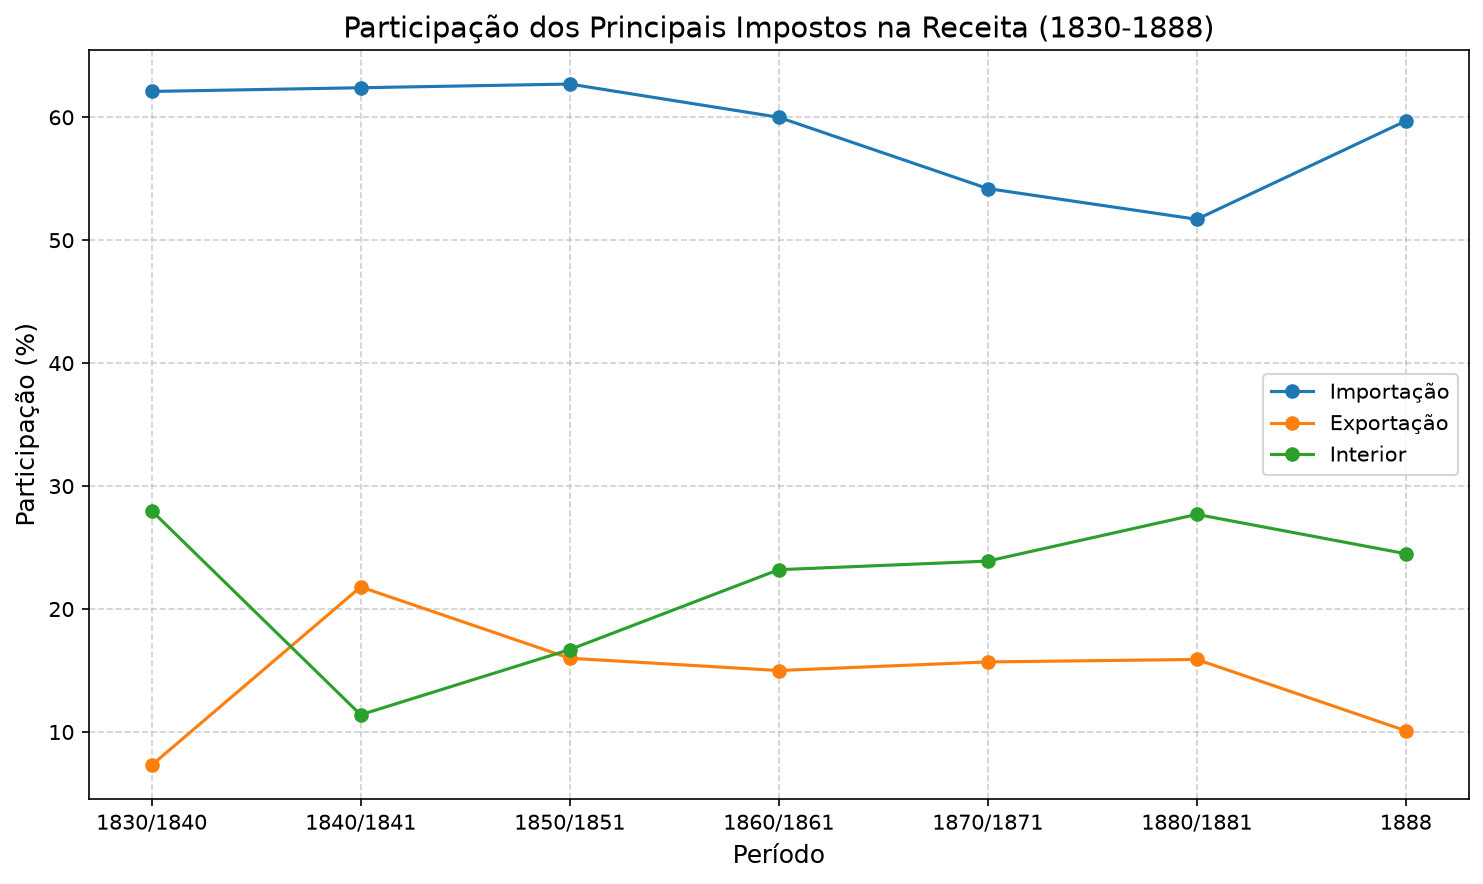
\includegraphics[width=\linewidth]{figures/cap04/impostos_participacao_1830_1888.png}
\caption{Participação relativa dos principais impostos na receita, 1830--1888 (mesmos dados da Tabela~\ref{tab:cap04-impostos-receita})}
\label{fig:cap04-impostos-participacao}
\end{figure}

Tal fato é, para Furtado
\citeyearpar{furtado2005}, mais
prejudicial ao desenvolvimento industrial brasileiro do que propriamente
a ausência de barreiras aduaneiras ou de outras formas de proteção da
indústria local. Inclusive, pois, na ausência de capacidade de
arrecadação, a emissão de moeda como recurso alternativo ao
financiamento do governo provocou forte desvalorização da moeda nacional
\citep{furtado2005}. Tal
desvalorização tem impacto sobre as populações urbanas e limitou a
capacidade de importação, tendo um efeito ``protecionista'' em certa
medida até superior ao que seria esperado de barreiras
aduaneiras típicas~\citep{furtado2005}.

\begin{figure}[htbp]
\centering
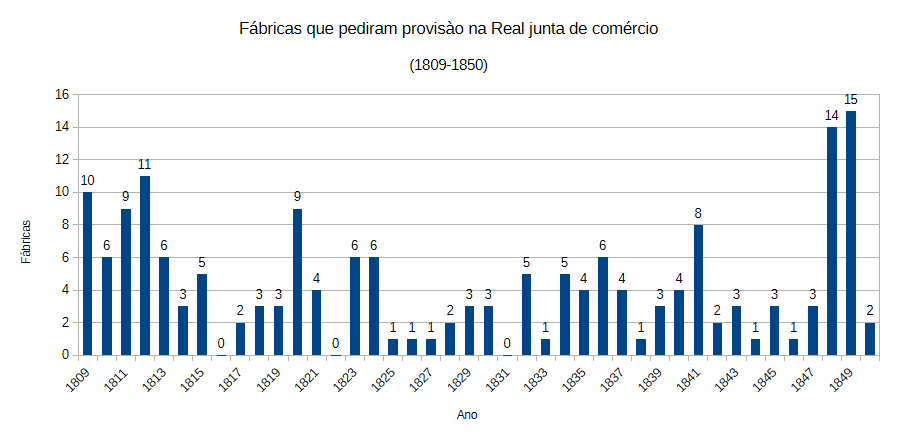
\includegraphics[width=\linewidth]{figures/cap04/grafico1-arrecadacao.png}
\caption{Fonte: Arquivo Nacional. Fundo da Real Junta de Comércio}
\end{figure}
\aiflag{Esta figura (grafico1-arrecadacao.png) parece não corresponder ao texto ao redor: o conteúdo real do gráfico é ``Fábricas que pediram provisão na Real Junta de Comércio (1809-1850)'' -- os mesmos dados de figures/cap04/fabricas\_1809\_1850.png (ambos derivados de tables/cap04/estatisticas\_secxix/industrias\_1809\_1850.csv) -- e não dados de arrecadação/impostos como o parágrafo discute. Falta também um \texttt{label} e uma legenda descritiva (hoje só a fonte). Considerar mover esta imagem para o ponto do texto sobre a relação com a indústria (ver marcador de tarefa mais adiante, ``Falar da relação com indústria'') e remover a duplicata.}

É preciso também apontar outro efeito importante da independência: a
formação da dívida externa brasileira. Em busca de apoio e
reconhecimento externo, o Brasil recém-independente precisará manter os
privilégios da Inglaterra. A formalização do reconhecimento da
independência vem, em 1825, com a delimitação também do pagamento de
dois milhões de libras aos ingleses \citep[]{tratado_da_paz_1825}. Esse acordo estabelecia
assim o ponto de partida da dívida externa brasileira, distinta de uma
dívida do reino português.

\aiflag{Ver Figura~\ref{fig:cap04-divida-externa} (inserida mais adiante no capítulo) -- optou-se por referenciá-la aqui em vez de duplicar a mesma imagem neste ponto. Conferir se não seria preferível deslocar a figura para cá, mais próxima da discussão sobre a formação da dívida externa.}

Ou seja, ao mesmo tempo que a independência eliminava um intermediário
oneroso, também pressionava o novo Estado a negociar diretamente com o
capital hegemônico, negando parte dos potenciais ganhos advindos da independência. =
Um sinal dessa fragilidade é o que Furtado
\citeyearpar[p.~145]{furtado2005} vai
denominar uma ``aplicação unilateral do liberalismo'' ao comentar os
privilégios concedidos à Inglaterra no comércio, sem contrapartida
equivalente. Mesmo que em 1827 tenha havido certa recuperação da
autonomia, com a não renovação do acordo de 1810, os privilégios
ingleses persistiram muito significativos até 1844
\citep{furtado2005}.

Também para Prado Júnior
\citeyearpar{pradojunior2012} os efeitos
econômicos dessa primeira metade do século XIX foram mais negativos que
positivos. A abertura dos portos em conjunto com uma forte
desvalorização monetária -- decorrente da necessidade de financiar o
Estado nascente para o qual a antiga burocracia portuguesa se transferiu
-- propiciará uma expansão do comércio exterior. Mas, em que pese os
ganhos da exportação, haverá déficit em conta-corrente compensado com
(mais) empréstimos públicos no exterior. O autor aponta como alguns
setores industriais incipientes tais quais siderurgia e têxtil serão
praticamente eliminados pelas importações inglesas e francesas. Além
disso, a importação de hábitos de consumo por parte da corte, refletida
agora nas elites nacionais, será restritiva ao processo de poupança,
argumento também observado em
Furtado\citeyearpar{furtado2005}.

Ao mesmo tempo, a nova administração pública contribuirá para alguns
avanços administrativos -- como a formação de forças armadas, educação
pública e infraestrutura -- porém trará consigo peso de setores
improdutivos. Assim, o Estado brasileiro permanecerá em déficit, tendo
no meio do século cerca de 40\% das suas receitas absorvidas pelo regime
da dívida, segundo Prado Jr
\citeyearpar{pradojunior2012}.

\todouser{}{Pegar dado déficits públicos}

Em contraponto ao privilégio dado ao setor exportador primário, foi
intensificada a pressão contra o tráfico de escravizados,
~\todouser{}{NOTA SOBRE TRÁFICO E Inglaterra}
~\footnote {Combate tráfico de escravos Inglaterra}
consequência direta da negociação com
os ingleses. Como já dito, escravidão não só constituia um forte
limitante a possibilidade de industrialização do país, como seu legado
permanecerá enquanto condicionante do capitalismo brasileiro muito tempo
após seu fim \citep{mello1982}. Ela era tanto impeditiva da formação de um mercado interno
\citep{furtado2005}, como
da absorção de tecnologias e novas técnicas
\citep{pradojunior2012},
implicando uma estagnação do desenvolvimento das forças produtivas e uma
vinculação do crescimento econômico quase inteiramente às variações de
preços de \emph{commodities} no mercado internacional.

Ao longo dessa primeira metade do século XIX as pressões inglesas contra
a escravidão irão crescer. Tal cenário se acentuará em 1850 com o fim do
tráfico de escravos -- já tentado via legislação desde 1831. Mesmo que o
efetivo fim da escravidão ainda estivesse longe, tal transformação
mudava significativamente o cenário ao impor às elites agrárias uma
restrição significativa de mão de obra
\citep{furtado2005,mello1982,pradojunior2012}. Apesar de advinda de pressão externa,
a proibição é provavelmente a desencadeadora das mais importantes transformações
internas do país.

\todouser{}{Discutir gráfico de escravidão}

\begin{figure}[htbp]
\centering
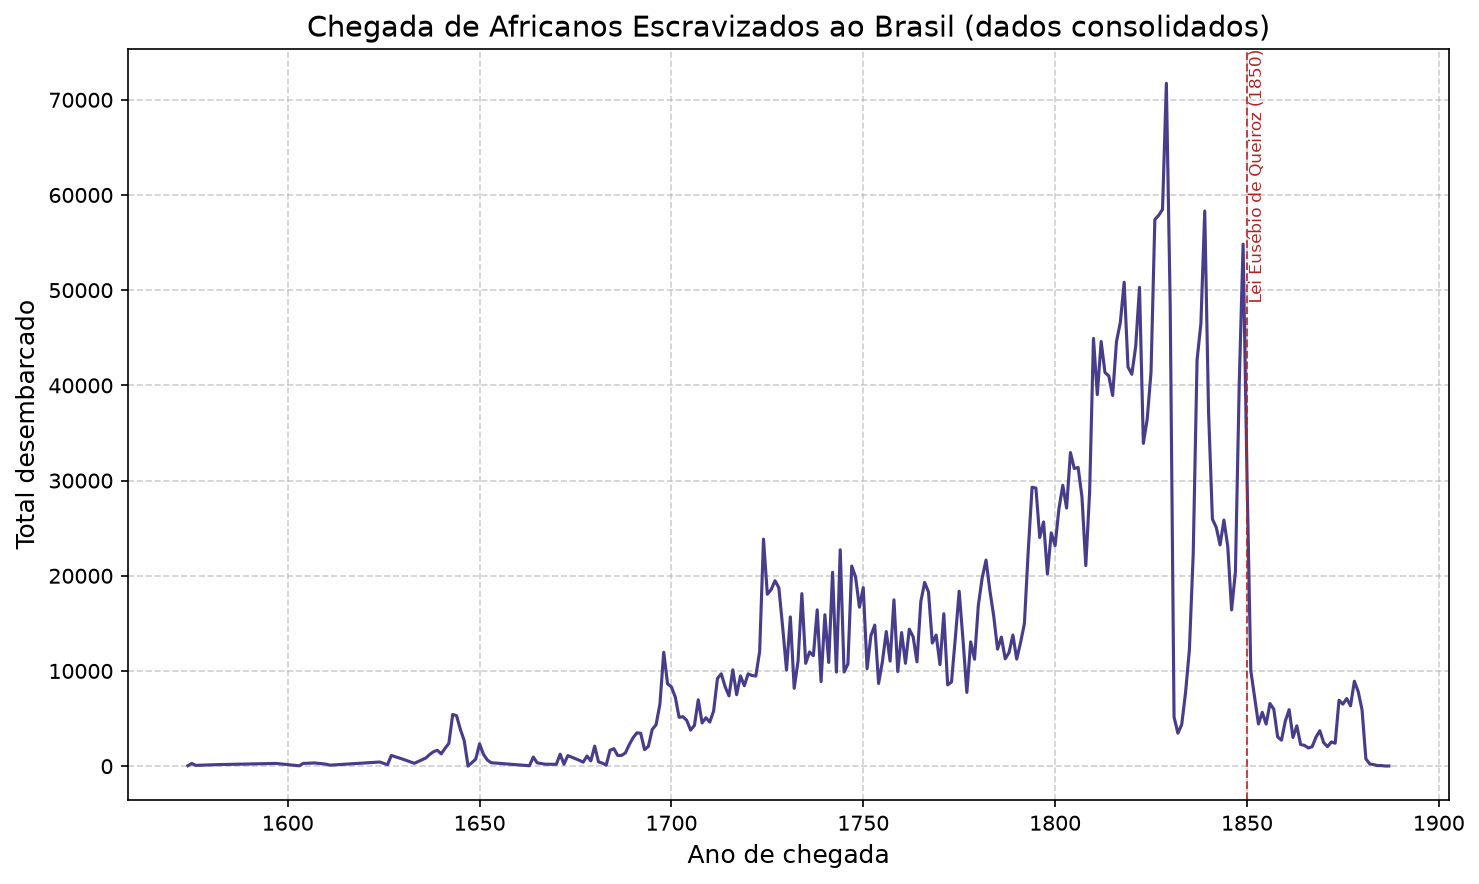
\includegraphics[width=\linewidth]{figures/cap04/chegada_escravos_slavevoyage_total.png}
\caption{Chegada de africanos escravizados ao Brasil, 1576--1888}
\label{fig:cap04-chegada-escravizados}
\aiflag{Fonte: slavevoyages.org (conferir citação bibliográfica adequada)}
\end{figure}
\aiflag{figures/cap04/chegada\_escravos\_slavevoyage.png, trafico-total.png e trafico-transatlantico.png parecem ser versões antigas/duplicadas deste mesmo gráfico (mesma série de slavevoyages.org, sem a anotação da Lei Eusébio de Queiroz e com eixos em inglês) e permanecem sem uso no capítulo -- considerar removê-las do repositório, a menos que tragam algum recorte de dado distinto (ex.: apenas tráfico transatlântico vs. total).}

Do ponto de vista da relação com os mercados externos, ao mesmo tempo,
começava a se gestar a indústria cafeeira. Esta já era presente desde os
anos 1830 e seria de fato o elemento re-integrador do Brasil nos
circuitos do comércio mundial após o declínio do açúcar
\citep{furtado2005}.
Ironicamente, o próprio setor cafeeiro em sua primeira fase utilizou em
larga escala a mão de obra escravizada, dando sobrevida a tal
instituição \citep{pradojunior2012}, mas seu crescimento se mostrava cada vez mais
incompatível com o uso dessa mão de obra, especialmente dadas as
restrições ao tráfico. Essa dupla pressão, uma integração via um produto
demandado externamente e uma restrição à força de trabalho até então
predominante vão operar a transformação da economia brasileira na
segunda metade do século XIX.

\todouser{}{Relacionar escravidão no setor cafeeiro com gráfico de escravidão}

Daí vê-se a contradição do caráter de dependência da economia nacional,
que sendo historicamente fruto de um condicionamento externo, exigia
justamente uma integração externa, porém condicionada a uma
transformação social interna, para poder avançar. A partir desse ponto
pode-se dizer também que essa dependência opera como um condicionante de
um desenvolvimento econômico propriamente capitalista,
~\footnote {Mello
  \citeyearpar{mello1982} separa a
  noção de uma economia colonial de uma economia primário-exportadora
  pela sua inserção na dinâmica global do capitalismo, na divisão
  internacional do trabalho. Rejeita assim a separação entre uma
  economia agrário-exportadora pré-capitalista -- com mão de obra
  escrava -- e capitalista -- com mão de obra assalariada -- apontando
  antes as continuidades entre ambos os arranjos no caso brasileiro,
  sendo a primeira um primeiro modo de inserção capitalista de países
  latino-americanos.},
não apenas pela inserção da economia mercantil
escravista na estrutura de acumulação do capital europeu, mas de fato
também pela internalização dos processos de decisão de investimento
\citep{mello1982}, em
contraponto a economia açucareira ainda orientada pelos interesses de
acumulação portugueses.

Dessa forma, o período não pode ser visto fora desse paradigma, de uma
economia já inserida num modelo capitalista que transitava a um
capitalismo monopolista, porém internamente ainda sem presença de forças
produtivas capitalistas
\citep{mello1982} --
veja: um mercado de trabalho assalariado e um capital fixo acumulado. A
organização de uma sociedade capitalista que possa internamente dar luz
a essas forças se dará apenas na segunda metade do século, mesmo que
algumas de suas pré-condições, em especial a constituição do Estado
nacional, o freio ao tráfico de escravizados e a gestação de uma
economia cafeeira capaz de acumulação de capital, já estivessem em
movimento.

\todouser{}{Falar da relação com indústria}
\aiflag{Sugestão de visualização: figures/cap04/fabricas\_1809\_1850.png (``Fábricas Autorizadas pela Real Junta de Comércio, 1809--1850'', dado em tables/cap04/estatisticas\_secxix/industrias\_1809\_1850.csv) está sem uso no capítulo e parece se encaixar bem neste ponto sobre a relação com a indústria nascente -- ver também a observação, mais acima, sobre a figura duplicada/mal posicionada (grafico1-arrecadacao.png).}

Mas, por hora, o Estado brasileiro ainda carecia de autonomia política
frente tanto em relação ao capital estrangeiro como em relação aos
interesses mais estreitos de suas elites. O país não contava com
capacidade de arrecadação, detinha uma população urbana -- agora cada
vez mais deslocada para o sudeste, com a \todouser{transferência da capital para o
Rio de Janeiro em 1831}{Inserir fonte} -- com consumo limitado pela desvalorização
monetária e uma força de trabalho constituída de escravizados empregados
em atividades intensivas, de baixa capacidade de absorção de tecnologia
e sem ganhos de produtividade. A atividade industrial que engatinhava
fora largamente eliminada pelas importações inglesas
\citep{pradojunior2012}
e a ``vocação agrícola'' do novo país parecia consolidada.

\section{A transformação na segunda metade do século XIX}\label{a-transformauxe7uxe3o-na-segunda-metade-do-suxe9culo-xix}

Como já dito, a segunda metade do século XIX será marcada por duas
transformações interligadas: a expansão do setor cafeeiro e o fim da
escravidão. Ambas representam transformações institucionais, no modelo
de acumulação e no mercado de trabalho respectivamente, diretamente
relacionadas à origem da industrialização nacional. No caso da primeira,
os \todouser{ciclos de preço do café}{inserir figura} \aiflag{nenhuma das imagens de preço do café disponíveis (figures/cap04/preco\_cafe\_1901\_1950.png, preco\_cafe\_1920\_1980.png, preco\_cafe\_1901\_2000.png) cobre o período discutido aqui (décadas de 1870-1890); todas começam em 1901. Falta produzir um gráfico específico para o século XIX -- ver specs/roadmap.md.}, associados aos longos períodos
de plantio e colheita, condicionam essa \textit{industrialização associada} a um ciclo de
expansão do capital cafeeiro. Este, utiliza desta expansão industrial para baratear a 
reprodução de sua força de trabalho e como oportunidade de investimento no momento da
realização dos lucros no mercado internacional
\citep{mello1982}.

Já o fim da escravidão, representa o ponto de partida para a formação de
um mercado de trabalho assalariado, estabelecendo uma relação de
produção efetivamente capitalista no Brasil
\citep{mello1982}. Prado
Jr. \citeyearpar{pradojunior2012} descreve
como a crise do sistema escravista não era apenas econômica, mas também
envolvia disputas entre forças políticas sociais impulsionadas pela
emancipação política. Isso, pois escravidão já não dispunha de uma
justificação moral aceita pelos atores em princípios do século XIX
\citep{pradojunior2012}.
Porém, a posição privilegiada que a elite rural, maior beneficiária do
sistema, assume após a independência, dificultou sua abolição. Isso se
refletia tanto na elite açucareira como nos cafeeiros escravistas, mas
foram os segundos que primordialmente sustentaram a economia
mercantil-escravista até a segunda metade do século
\citep{mello1982},
particularmente o café do Vale do Paraíba do Rio de Janeiro
~\todouser{}{Discutir gráfico de escravidão}. Esse
movimento já era sinal do deslocamento do eixo econômico do Nordeste
açucareiro para o Sudeste cafeeiro, a despeito do fraco crescimento
vegetativo da população escravizada, e que se consolida com o café do Oeste
Paulista na segunda metade do século.

A perpetuação da escravidão representa um caso de uma elite cuja posição de poder
permite uma busca de interesse próprio que não é necessariamente
condizente com um ``interesse comum'', o que é condizente com a literatura
sobre o papel de elites econômicas no desenvolvimento \citep[]{amsdenRoleElitesEconomic2012}.
Esse certo caráter ``rentista'' da elite agrária escravista Furtado
\citeyearpar{furtado2005} associa a sua
exclusão da esfera do comércio e restrição pelo domínio comercial
inglês, ficando esta restrita a um papel produtivo isolado. Essa elite
se torna assim obstrutora de transformações institucionais que já à
época eram consideradas inevitáveis. A solução mediada pelos atores
contemporâneos foi a concepção da escravidão como um ``mal temporário''
\citep{pradojunior2012},
o que evidencia tanto o gradual declínio dessa instituição, como as
dificuldades de se operar sua substituição em meio aos interesses
correntes.

Mas se apenas o processo de formação de uma nova nação não era
suficiente, apesar de contributivo, para o declínio da escravidão, a
pressão externa contribuirá para este. A pressão inglesa através do
combate ao tráfico negreiro, que alcança seu ápice em 1845 com a
declaração de Bill Aberdeen autorizando a apreensão de qualquer
embarcação que traficasse escravizados
\citep{pradojunior2012}, o que causará significativo desajuste da ordem econômica
brasileira.

Tal pressão externa interage com um parcial rearranjo interno das
elites. Prado Jr.
\citep{pradojunior2012}
aponta como a ascensão econômica dos traficantes de escravos colocava a
própria elite agrária em posição favorável a certa restrição do tráfico,
receosa de perder sua posição dominante. Assim, adota-se uma estratégia
de preservação do poder econômico-político por graduais
concessões à restrição do tráfico escravagista, que culminam na sua
total proibição em 1850. Em que pesem picos de chegadas de escravizados,
justamente tentativas de obter mão de obra antes da proibição
considerada questão de tempo, a entrada de escravizados se reduz quase
que por inteiro entre o segundo e terceiro quartil do século XIX (ver Figura~\ref{fig:cap04-chegada-escravizados}).

Para além da normalização das relações com os ingleses -- que implica
uma retomada da entrada de capitais estrangeiros no país --, o fim do
tráfico de escravizados implica uma ``liberação de capital'' para
diversas outras atividades econômicas
\citep{pradojunior2012}. 
que parece coincidir com a formação de diversos mercados de capitais no
país (Musacchio, 2009 \emph{apud} \citeauthor{pereira_dos_santos_formation_2024}, \citeyear{pereira_dos_santos_formation_2024}).
Esse processo tanto servirá para constituição de
importantes empreendimentos de infraestrutura \cite{saraiva_atlas_nodate}, como para adoção
de modelos institucionais modernos, como o sistema de responsabilidade
limitada e a formação da bolsa de valores do Rio de Janeiro
\cite{levyHistoriaBolsaValores1977}. O significativo crescimento das caixas econômicas e bancos
também apontam nesse sentido \cite{saraiva_atlas_nodate} \ref{fig:cap04-bancos-criados}.

\begin{figure}[htbp]
\centering
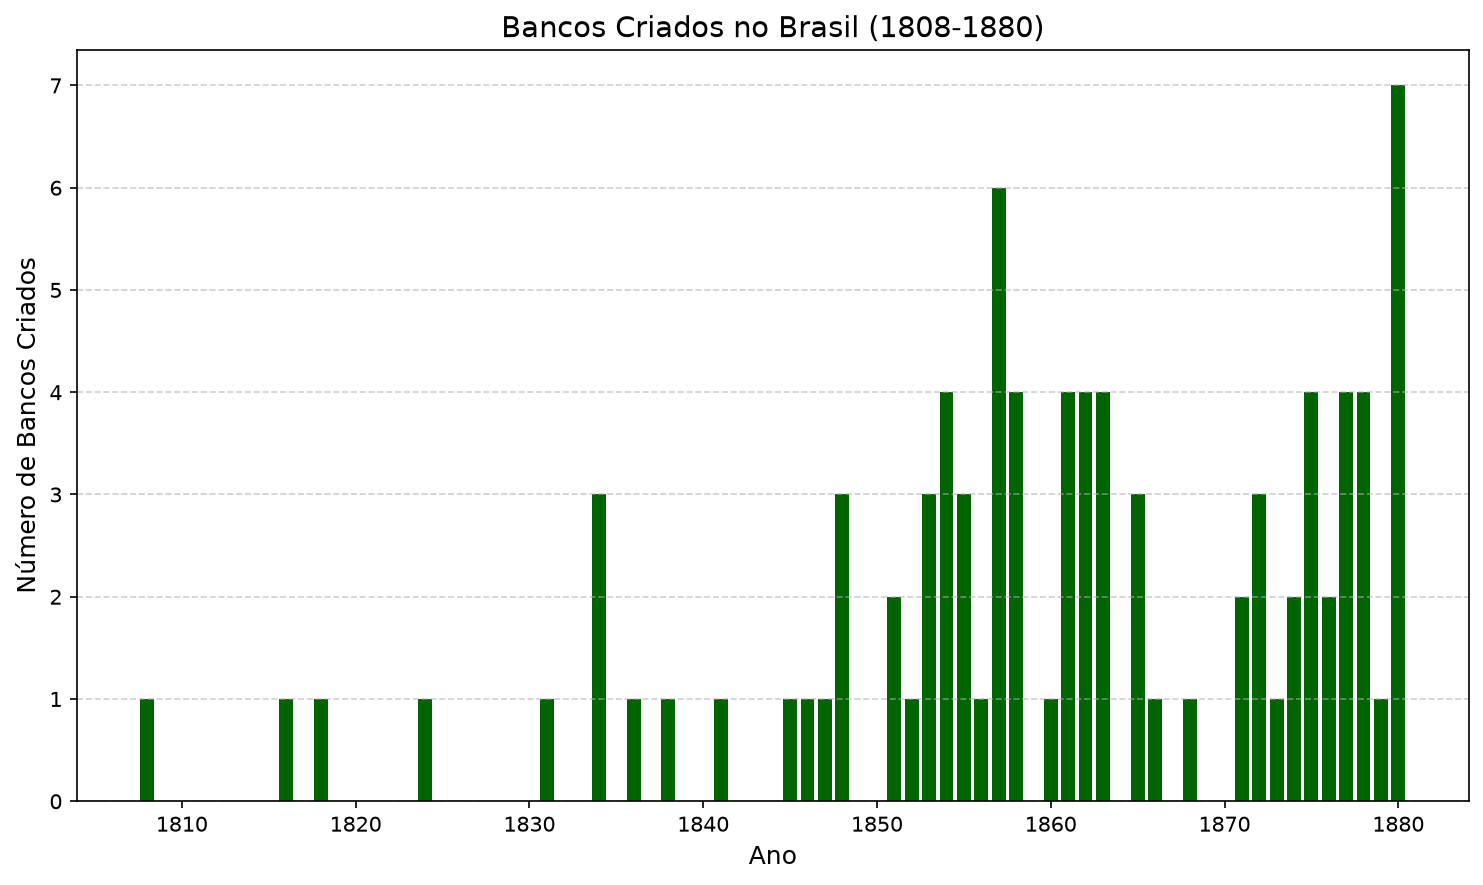
\includegraphics[width=\linewidth]{figures/cap04/bancos_criados_1808_1880.png}
\caption{Bancos criados no Brasil, 1808--1880 Fonte: \citep{mello2008}}
\label{fig:cap04-bancos-criados}
\end{figure}
\aiflag{figures/cap04/figura1-modernizacao-financeira.png parece ser um mesmo gráfico ``Bancos Criados (1808--1880)'' duplicado (mesmos dados, estilo diferente) e permanece sem uso no capítulo -- considerar removê-lo do repositório de figuras para evitar redundância, a menos que haja diferença de dados não percebida pela IA.}

\begin{table}[htbp]
\centering
\caption{Valores depositados nas caixas econômicas por província, 1889}
\label{tab:cap04-depositos-caixa}
\csvautotabular{tables/cap04/estatisticas_secxix/depositos_caixa_econ_1889.csv}
\end{table}

\begin{figure}[htbp]
\centering
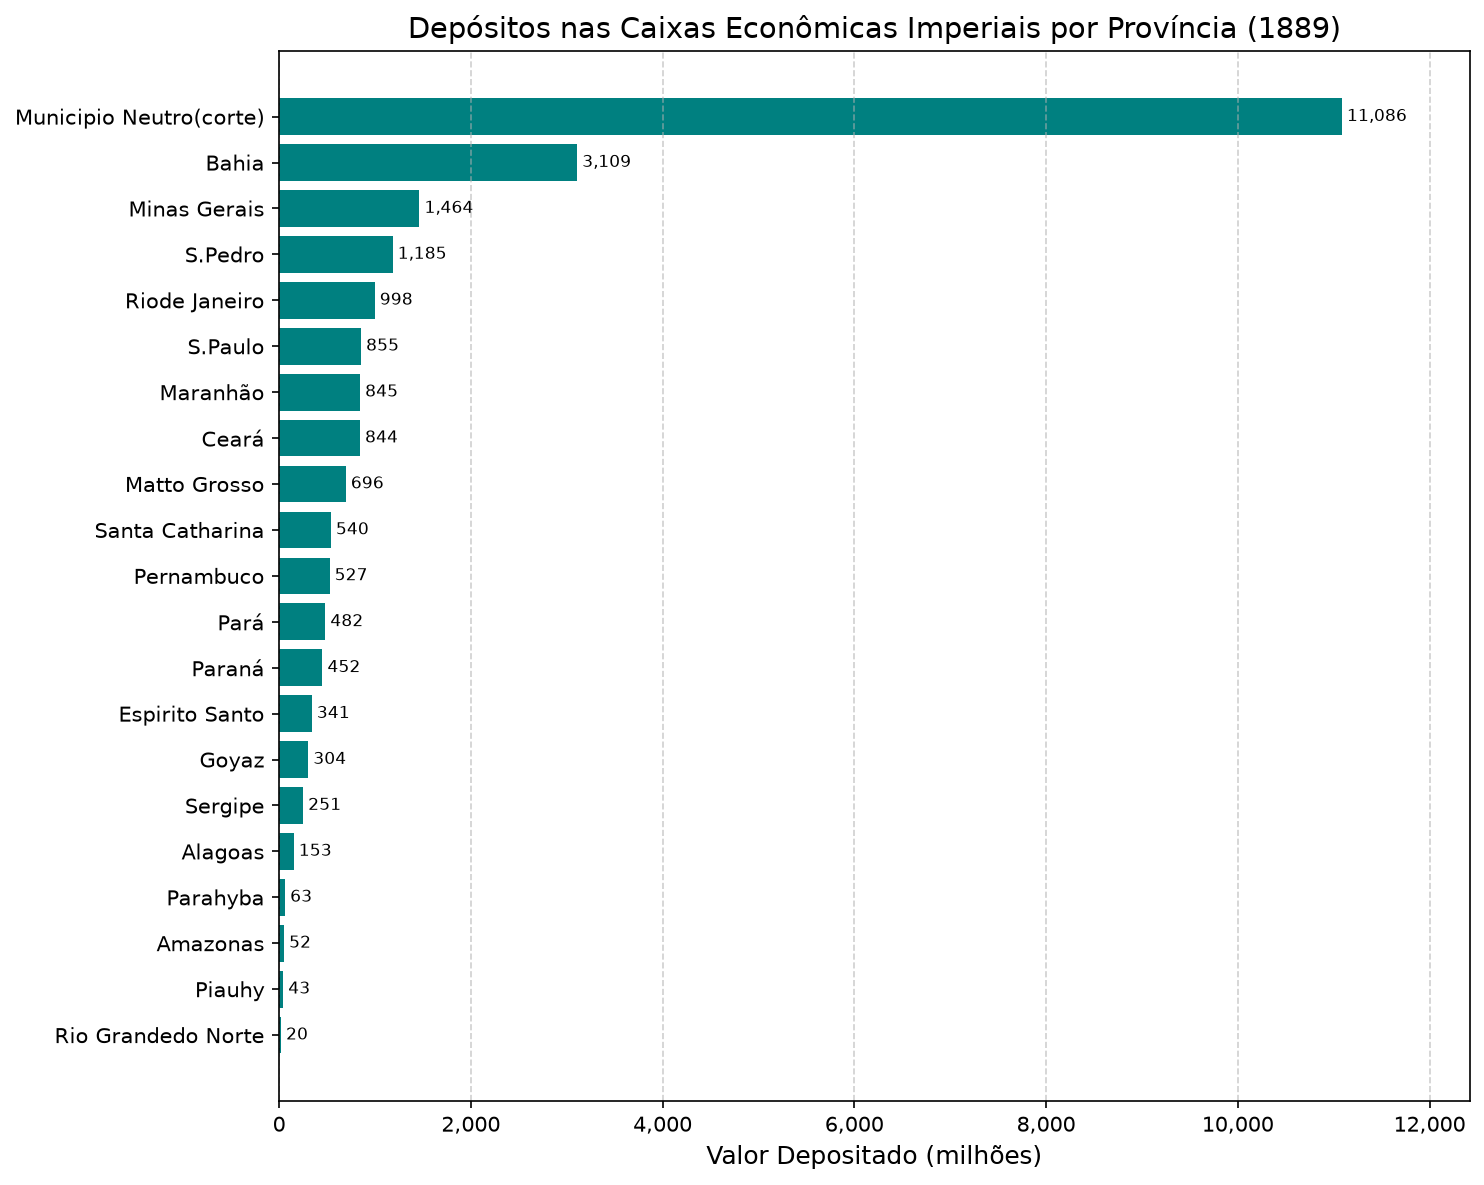
\includegraphics[width=\linewidth]{figures/cap04/depositos_caixa_econ_1889.png}
\caption{Depósitos nas caixas econômicas por província, 1889}
\label{fig:cap04-depositos-caixa}
\aiflag{(fonte)}
\end{figure}

Entretanto, tal ``modernização'' da economia brasileira será desafiada e
limitada por importantes fatores: a baixa produtividade e a escassez de
mão de obra. Não à toa a liberação de capital proveniente do fim da
escravidão se concretiza também em forte pressão inflacionária
\citep{pradojunior2012}. Sobre o primeiro fator, Furtado
\citeyearpar{furtado2005} já apontava a
significativa dependência tecnológica brasileira na época. Ao mesmo
tempo, havia baixo crescimento vegetativo da população escravizada
\citep{pradojunior2012},
exemplificando as condições extremamente precárias às quais tal
população era submetida. Isso implicava uma dependência externa para o
crescimento do país em termos de poupança -- baseada na formação de
dívida externa -- mão de obra -- respondida primeiramente via escravidão
e depois, como será visto, via imigração -- e tecnologia. Os ciclos de
preços do café, ligado ao descompasso da produção com limites da demanda
e a presença de produtos substitutos, também impactaram fortemente a
economia, demonstrando claros limites do setor cafeeiro escravista em
prosseguir sua expansão sem significativas transformações
\citep{mello1982}.

Portanto, como condição para a expansão cafeeira era preciso solucionar
a questão da mão de obra. Isso será possível, entretanto, devido à
característica que o café assume comparado aos demais empreendimentos
exportadores nacionais até então. Mello
\citeyearpar{mello1982} mostra
que o café já era uma grande empresa escravista de capital nacional e
articulada num sistema comercial-financeiro nacional. Assim, apesar da
imposição do trabalho escravo ter advindo da natureza colonial
exportadora, não se deve perder de vista que ali já se constitua uma
economia nacional que, com a formação de um Estado nacional, propiciava
que se ``nacionalizasse a apropriação do excedente e se internalizassem
as decisões de
investir''~\citep[p.~58]{mello1982}. Essa nova elite se beneficiava de uma atividade menos
intensiva em capital que o açúcar e, diferente da elite açucareira,
estava diretamente relacionada ao comércio de seu produto. Assim,
poderia com mais facilidade operar como classe, uma ação coletiva que
utilizava o governo como instrumento e que posteriormente se
beneficiaria largamente da descentralização política resultante da
autonomia dos estados com a proclamação da república
\citep{furtado2005}.

Por sua vez, o deslocamento do setor cafeeiro do Vale do Paraíba para
São Paulo, que no último quartil de século se torna o maior produtor de
café, é explicado tanto pelo esgotamento das terras da região fluminense,
em função do uso de técnicas extensivas e pouco apropriadas a preservação do solo,
como viabilizado pelas inovações de transporte, como a estrada de ferro
que vinha a reboque do capital inglês
\citep{mello1982}. Essa melhoria no sistema de transporte possibilita acesso
ao Oeste-Paulista, de terras e relevo mais favoráveis ao plantio de café
\citep{pradojunior2012}.
E é em São Paulo que se introduziu a máquina para beneficiamento de café
nos anos 1870, permitindo a melhora de preços associada ao produto de
mais qualidade, que sustentará o crescimento do setor cafeeiro
\citep{mello1982} ~\todouser{}{INSERIR GRÁFICO CAFÉ} \aiflag{mesma lacuna já apontada acima -- nenhuma imagem de preço do café disponível cobre os anos 1870, período desta passagem (máquina de beneficiamento em São Paulo).}. Também
contribui para a elevação dos preços a busca americana pelo café brasileiro, em lugar do café
indiano de dominação britânica
\citep{pradojunior2012}.

Dessa maneira, foi através desse setor cafeeiro do Oeste paulista, cada
vez mais representativo das exportações brasileiras (FIGURA \ref{tab:cap04-exportacoes}), que se
desenvolveram esforços de solução do problema, mas não sem lhes infundir
com uma visão eugenista predominante à época. Diante da expansão
cafeeira e cada vez mais restrita à obtenção de escravizados, a
imigração foi priorizada como modelo de abastecimento de mão de obra
para o setor cafeeiro
\citep{furtado2005,mello1982,pradojunior2012}.

\begin{table}[htbp]
\centering
\small
\caption{Exportações Brasileiras, 1820--1890 (em milhões de libras esterlinas)}
\label{tab:cap04-exportacoes}
\csvautotabular{tables/cap04/exportacoes-1820-1890.csv}
\caption{Fonte: \citep[p.~342]{nogueira1988}}
\footnotesize *O item ``Outros'' consistia em produtos como erva-mate, diamante, ouro,
castanha do Pará, madeiras, farinha de mandioca, aguardente e outros
produtos, sobre os quais não se dispõe de informações estatísticas
confiáveis.
\end{table}

\begin{figure}[htbp]
\centering
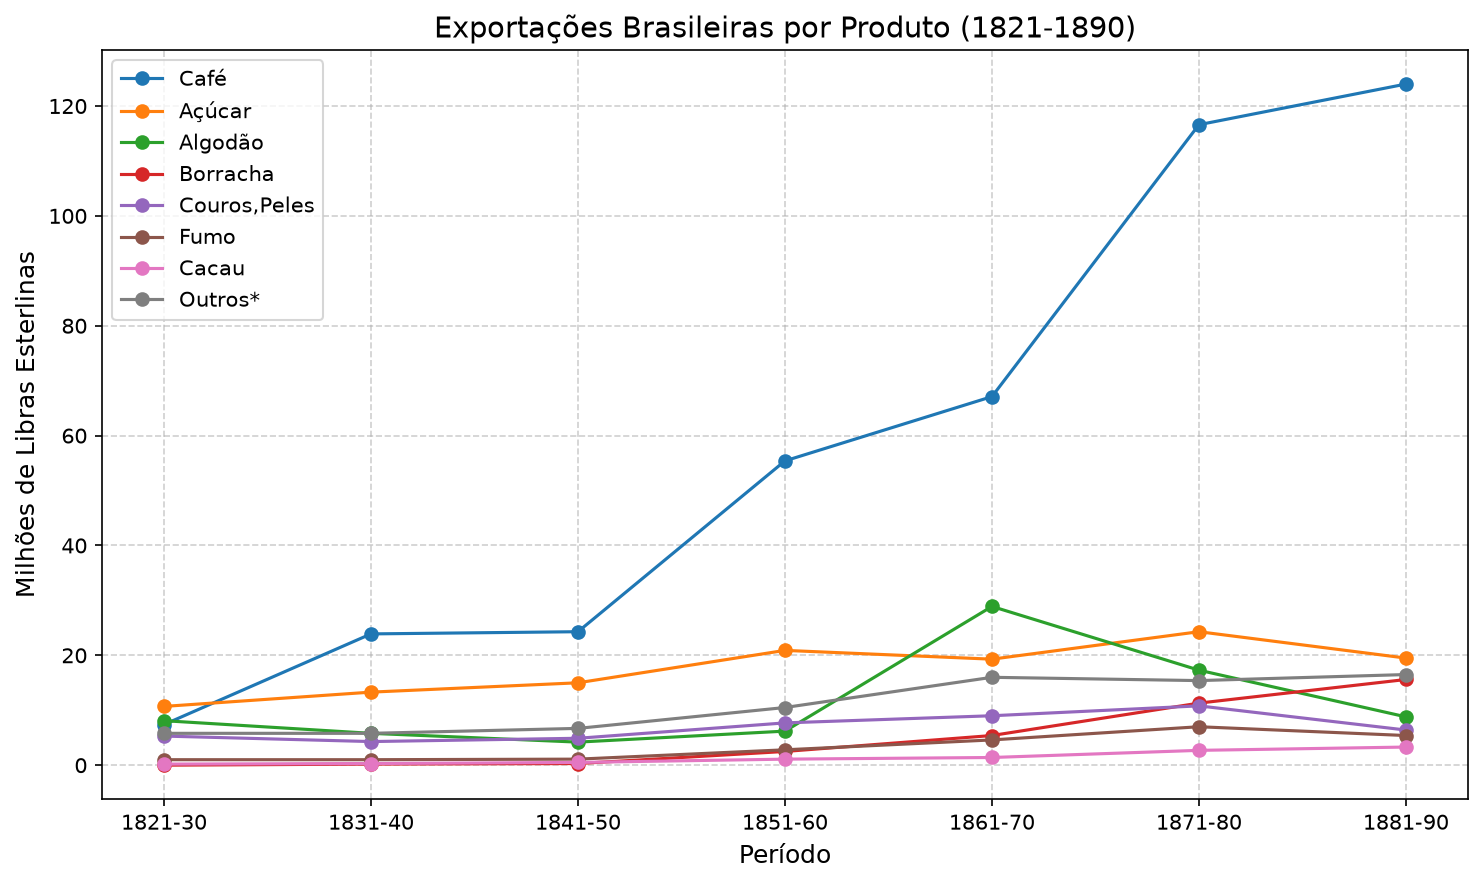
\includegraphics[width=\linewidth]{figures/cap04/exportacoes_por_produto_1821_1890.png}
\caption{Composição das exportações brasileiras por produto, 1821--1890 (mesmos dados da Tabela~\ref{tab:cap04-exportacoes})}
\label{fig:cap04-exportacoes-produto}
\end{figure}

Aqui, em que pese todas as limitações econômicas relativas à utilização
de uma mão de obra que passou pelo processo de escravização -- em
especial a tendência sua superexploração que desestimulava os patrões a
adotarem melhorias em técnicas produtivas
\citep{mello1982} -- é
preciso não considerar como de menor importância o critério racial na
escolha de uma política de imigração. Sinal disso é que o esforço
estatal em prol do processo de imigração precede seu uso no setor
cafeeiro, em parte movida por esforços de branqueamento da população e
em parte pela tentativa de mímica da experiência americana. \aiflag{sugestão de citação: a afirmação sobre a política de imigração como projeto de ``branqueamento'' é uma tese historiográfica específica (associada normalmente a autores como Skidmore) e está sem citação direta neste trecho -- avaliar se references.bib já cobre essa literatura ou se falta incluir uma fonte.}

Tal tentativa prévia, entretanto, havia sido malfadada, como aponta Furtado
\citep{furtado2005}.
Entre os colonos que visavam ocupação do território, como no Rio Grande do
Sul, encontravam em território brasileiro pouco mercado consumidor para
seus excedentes produtivos, tendo eles baixo crescimento vegetativo e
pouco espaço para acumulação. Já aqueles que vinham para trabalhar na
grande lavoura encontravam condições muito mais precárias que no Norte
dos Estados Unidos. Mesmo o intermédio direto dos plantadores de café,
buscando sanar sua necessidade de mão de obra foi insuficiente, pois as
condições oferecidas aos imigrantes, principalmente o estabelecimento de
dívida com o senhor de terras, acabavam por degenerar o modelo de
trabalho para similar ao regime de servidão
\citep{furtado2005}.

\aiflag{[FIGURA A INSERIR: GRÁFICO POPULACAO IMIGRANTE]}

\begin{figure}[htbp]
\centering
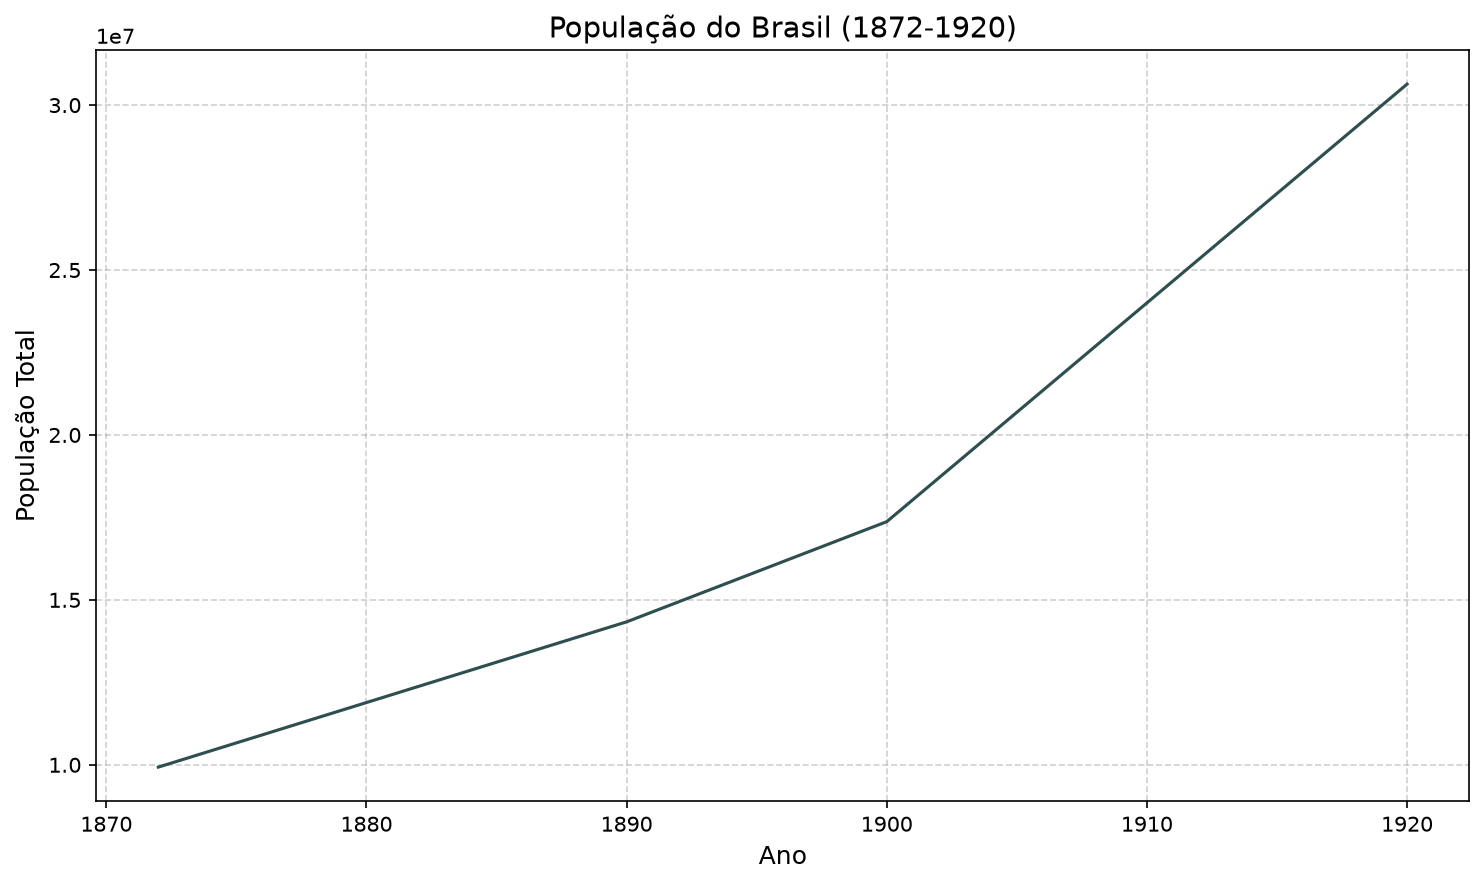
\includegraphics[width=\linewidth]{figures/cap04/populacao_1872_1920.png}
\caption{População total do Brasil, 1872--1920}
\label{fig:cap04-populacao-total}
\aiflag{(fonte) -- atenção: esta é a única imagem de população não utilizada no capítulo, mas é população total do Brasil por censo, não especificamente população imigrante como pede o marcador acima. Mantida aqui como aproximação do crescimento demográfico do período; se o autor quiser um gráfico específico de entrada de imigrantes, o dado ainda precisa ser produzido (ver specs/roadmap.md).}
\end{figure}

A solução definitiva do problema da mão de obra exigiu significativos esforços estatais,
tanto do ponto de vista financeiro como na construção institucional de um mercado
de trabalho capaz de melhor absorver esse imigrante. Esse problema era prioridade, pois 
o Estado brasileiro
continuava precisando refinanciar sua dívida externa e profundamente
dependente do setor exportador
\citep{pradojunior2012}.
Assim, o Estado que já tinha tentado sem tanto sucesso o modelo de
imigração para colonização na região Sul, passou a atuar conjuntamente
com os esforços privados na tarefa de produzir uma solução para a falta
de mão de obra para o café
\citep{pradojunior2012}.

Furtado \citep{furtado2005} descreve essa solução como um sistema de pagamento baseado na
parceria entre colono e proprietário adicionado de um pagamento fixo.
Com isso, o contratante absorve parte do risco do colono. Adicionalmente, a partir de
1870 o governo arca com custos da viagem e primeiro ano do colono, o que
serve para reduzir os riscos de servidão por dívida, além da
garantia de terra para plantio de subsistência. Esse conjunto de
inovações institucionais, somadas a já citadas melhorias em meios de transporte
\citep{pradojunior2012},
tornam o mercado de trabalho brasileiro novamente atraente para o colono,
especialmente num cenário de escassez de terra após a unificação
italiana \citep{furtado2005}.

Tal tratamento diferenciado ao imigrante europeu contrastava com uma
oferta de mão de obra no Nordeste não utilizada. Esta, ao invés de
inicialmente imigrar para o Sudeste -- o que apenas se dará apenas
posteriormente -- foi destinada à indústria da borracha na região Norte,
na bacia amazônica, sob condições muito inferiores àquelas oferecidas
aos imigrantes europeus
\citep{furtado2005}. De
fato, ali muitas vezes o regime de dívida implicou a formação de um
regime de servidão, justamente fator ao qual a ação estatal precisou
conter no Sudeste.

A borracha tem também importância simbólica ao demonstrar uma integração
da economia nacional com demandas específicas das novas atividades
industriais, reforçando o ponto de Mello
\citep{mello1982} sobre a
relação entre economias periféricas exportadoras de matéria-prima e
desenvolvimento do capitalismo. Foi a combinação de processos de seca --
especialmente entre 1877 e 1880
\citep{furtado2005} -- e a 
demanda de terras para plantio do algodão que expulsaram trabalhadores
do campo no nordeste, mão de obra que seria absorvida no Norte. Mas
oposto ao que ocorreu na revolução industrial europeia, essa mão de obra
não se direcionou às cidades e nem a atividade industrial diretamente,
mas sim ao fornecimento de matéria-prima para esta, ressaltando que
mesmo em processos de expulsão do campo a relação de dependência
condiciona os resultados. Também diferente do caso da indústria
cafeeira, a indústria da borracha terá um ciclo mais curto, declinando com entrada no mercado
internacional da borracha vindas do oriente, resultando numa mão de
obra subutilizada na região
\citep{furtado2005}.

Assim, o caso brasileiro mostra novamente como a relação entre uma elite
local e uma demanda global -- por algodão e borracha no caso -- pode não
conduzir a uma capacidade de acumulação de capital endógena e nem formar
mercados consumidores. Se nas economias centrais ou mesmo no sudeste
havia maiores incentivos à alocação da população em atividades mais
produtivas, inclusive aí a capacidade de apoiar uma reprodução social de
maior custo, no Norte e Nordeste predominou a subutilização dessa mão de
obra.

Furtado \citeyearpar{furtado2005}
enfatiza essa diferença também nos efeitos do fim da escravidão. Se no
setor açucareiro a falta de terras levou a população ao trabalho
assalariado de baixa renda -- nível de subsistência -- no setor cafeeiro
a relativa disponibilidade de terras para subsistência forçou uma
elevação de salários frente ao risco de perda da mão de obra necessária
ao setor cafeeiro. Esse fator foi intensificado pela concorrência do
açúcar cubano e modificações técnicas nos engenhos de açúcar que
reduziram a demanda de mão de obra anteriormente a libertação dos
escravizados, implicando numa reduzida distribuição da renda no mercado
nordestino comparado ao sudeste.

No caso do sudeste, além da maior oferta de terras, a infraestrutura
local facilitava o uso produtivo de terras mais afastadas. O resultado
foi uma distribuição da renda em favor do trabalho justamente no
território de imigração Europeia, branca. Não é de se estranhar então
o predomínio do crescimento econômico no sudeste e a 
marginalização de longa data tanto da população negra descendente de
escravizados como da população nordestina, que continuará por bom tempo
operando como reserva de mão de obra de baixo custo do sudeste \todouser{}{INSERIR FONTE (Paulo Fontes?)}.

Vale aqui pontuar que, durante todo esse período, predominou na elite
brasileira uma concepção de ``vocação agrícola'' do país \citep{curado_industrializacao_2013}.
Isso não implica a inexistência de um pensamento industrializador ou de
associações de classe industrial, como Barreto \citeyearpar{barreto_o_2018} mostra no caso do
Rio de Janeiro. Entretanto, havia forte orientação à atividade agrícola,
considerada inclusive a impulsionadora da capacidade industrial
\citep{barreto_o_2018} e um claro domínio 
político das elites rurais -- especialmente as escravistas até o fim do império. 
Era uma expressão ideológica que via a indústria não como substitutiva ou 
etapa posterior, mas como reflexo -- positivo, mas reflexo -- da prosperidade 
advinda do campo.

Se a discussão acima parece ter tergiversado sobre nosso desenvolvimento
industrial, enfatizando questões prévias a este, é importante apontar a
significativa importância dos eventos narrados a interpretações do
período industrializante -- e desindustrializante -- da economia
brasileira.

Como já dito, um argumento que transpassa o texto é que a dinâmica entre
uma agricultura voltada à exportação e a imposição externa de um sistema
escravocrata são não uma forma pré-capitalista, mas, um arranjo de
expansão capitalista na periferia voltado ao processo de acumulação
primitiva do centro, como proposto por dependencistas como \todouser{Gunder Frank }{Pegar fonte}
e aqui mobilizado em Mello \citeyearpar[]{mello1982}. A
partir daí, o autor pensa o processo de formação da mão de obra
assalariada e industrialização do Brasil como condicionados por essa
trajetória escravocrata. O argumento que se apresentará futuramente é
que a própria desindustrialização brasileira também não poderá ser vista
como um rompimento com o período anterior e sim condicionada pela
característica da própria industrialização e, portanto, atrelada às condições de
sua origem. A distinção do processo de desindustrialização em um país
profundamente desigual e com mercado de trabalho altamente dualizado
para aquela ocorrida em mercados onde uma classe média maior já se
constituía -- como EUA ou Europa -- não pode ser minimizada.

Demonstra-se, também, a dependência de trajetória que implicará uma
concentração da atividade econômica no sudeste. Os dois pontos mais
importantes são a respeito da atividade exportadora cafeeira e da
formação de um mercado de consumo na região sudeste. Um deslocamento de
populações evidenciando uma mão de obra alocada em setor de maior
produtividade -- na maior parte dependente de preços do exterior --, mas
cuja elasticidade impedia o crescimento dos salários e amparava a
acumulação cafeeira
\citep{furtado2005}.

Além disso, a concentração política e de capitais no Rio de Janeiro pela
transferência da capital estruturam a região sudeste como local
privilegiado de investimentos em infraestrutura. Essa junção de fatores
será significativo impulso na industrialização ocorrida no período
seguinte -- de 1892 até 1929 -- e pode ser vista na concentração de
atividades industriais na região. É primeiro no Rio de Janeiro -- da
sede do governo, da concentração de capitais, da demanda de consumo
urbano e em algum grau do setor cafeeiro do Vale do Paraíba 
\cite{pedreira_historiografia_2024,barreto_o_2018} -- e gradualmente no estado de São Paulo, que se desenvolve o
primeiro impulso da indústria brasileira. Mais de cem anos depois, ambos
os estados continuam como os maiores parques industriais. São
também dois dos maiores locus de desindustrialização, como será visto nos
capítulos posteriores.

Não se trata aqui de um determinismo geográfico, onde a característica
do solo implicam a trajetória econômica do país. Como dito, as condições
de viabilidade econômica das terras do Oeste Paulista dependiam desde uma 
significativa infraestrutura de construção humana até uma exaustão das terras do
Vale do Paraíba relativa não a sua natureza, mas ao modo de uso da
mesma. Além disso, setores exportadores primários, como o açucareiro e o
da borracha, também produziram significativos excedentes de capital sem
que tivessem dado o mesmo impulso ao processo de industrialização. Foi a transformação da
classe cafeeira, num processo particular e historicamente determinado
pelo contexto de transformações institucionais políticas, que propiciou
um processo de diversificação do capital cafeeiro em atividades
industriais.

Tão pouco se pode relegar esse desenvolvimento a forças de mercado ou meros fatores
externos. Apesar do argumento correto de Suzigan \citeyearpar{suzigan_industrializacao_2000}, 
de que havia pouca intencionalidade ou participação estatal direta na industrialização
antes de 1930, não é correto dizer que o Estado e governo não foram relevantes para
industrialização desse período. O Estado foi essencial na constituição de mercado
de consumo e na mão de obra que puderam ser aproveitados pelo capital industrial nascente.
Isso para além de manutenção da capacidade de consumo com apoio do café, especialmente após 1930.
Que o crescimento quantitativo da indústria seja tímido até os anos 1930, não ignora que transformações
prévias constituam-se em fatores necessários, mesmo que não suficientes, a industrialização.

Há aqui também a ``história de origem'' de uma instituição que será
recorrente personagem na trajetória de desenvolvimento econômico
brasileiro, a sua dívida externa. Mais do que em países do centro
capitalista, no Brasil -- e América Latina -- a atividade industrial
terá um papel dúbio em relação à dependência financeira externa. Ela será
ao mesmo tempo, fruto de processos de endividamento externo e das
exportações, mas almejada como substitutiva dos processos de importação.
Daí também a relação intrínseca e continuada entre uma indústria
importadora de matérias-primas, maquinário e tecnologia e um setor agro
exportador de commodities, gerador de divisas externas.

\begin{figure}[htbp]
\centering
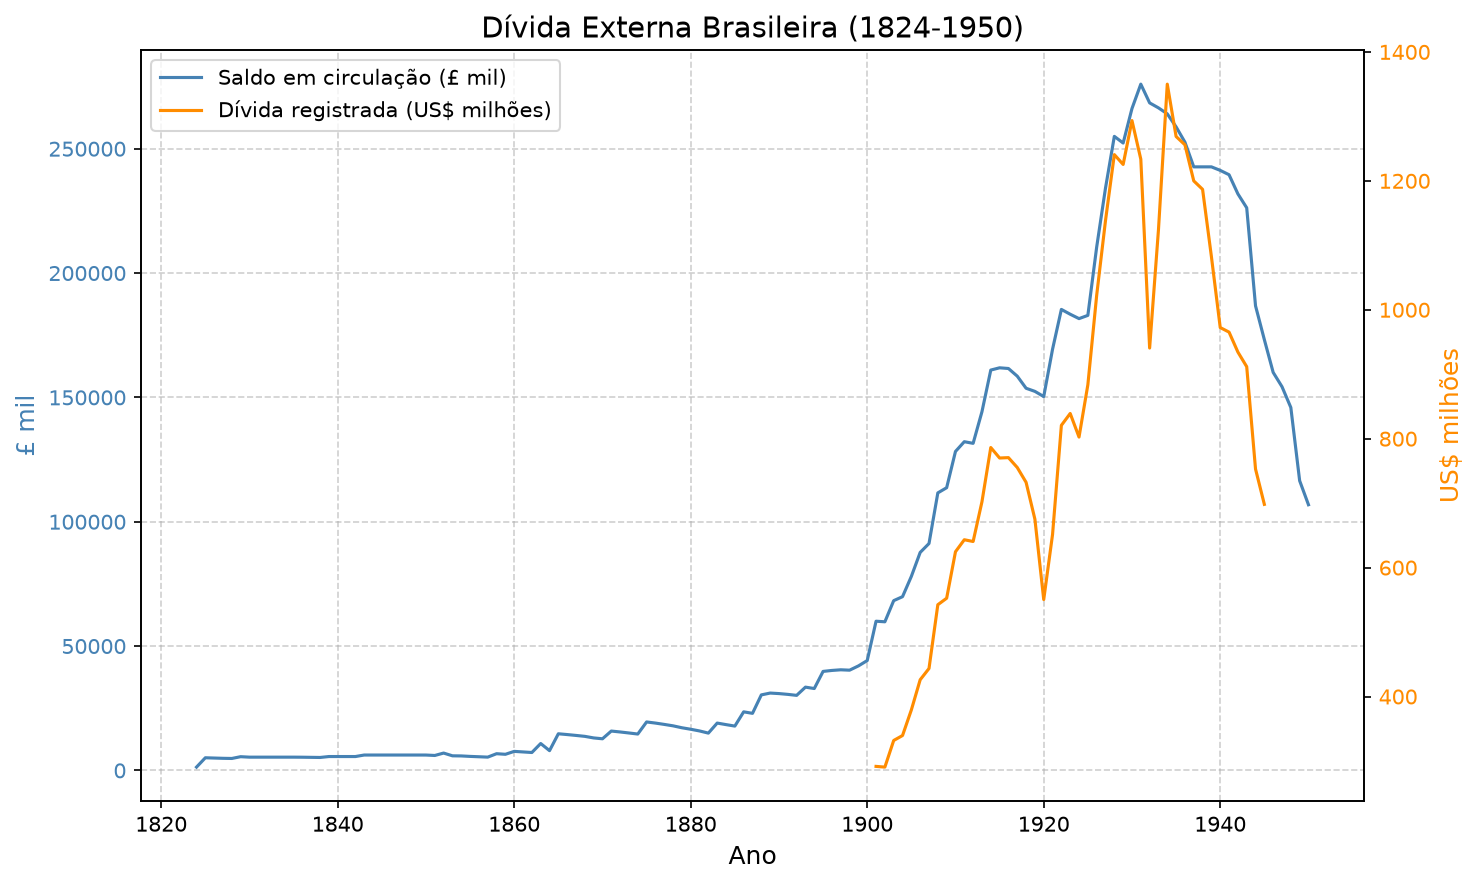
\includegraphics[width=\linewidth]{figures/cap04/divida_externa_1824_1950.png}
\caption{Dívida externa brasileira, 1824--1950}
\label{fig:cap04-divida-externa}
\todouser{fonte}{MARCAR Estatísticas século XX}
\end{figure}

Por fim, a elite rural será importante personagem em toda história. Sua
relação com as frações industrialistas brasileiras sempre será
reticente, apoiando sem renunciar a uma primazia de seu modelo de
acumulação. Isso não implica que esta elite seja monolítica ou estanque.
Apesar de ter evitado a ascensão política da classe de traficantes de
escravos \citep{furtado_formacao_2005}, as elites rurais escravistas acabaram em parte sendo
substituídas e em parte transformadas nas elites cafeeiras utilizadoras
de mão de obra assalariada. Neste terreno se dá uma junção de
abolicionismo com o imigrantismo
\citep{mello1982}. Ao
mesmo tempo, o abolicionismo toma força também em estados não cafeeiros,
cuja mão de obra escrava tinha sido ``drenada'' para as primeiras
plantações de café
\citep{mello1982}.

Soluções intermediárias foram tentadas ao longo das décadas para
conciliar reformadores abolicionistas e conservadores escravagistas,
como a libertação de nascituros, mas foram meros adiamentos do inevitável,
pois cresciam junto as pressões advindas de abolicionistas e revoltas escravas, fortalecidos
pela presença de mão de obra livre decorrente da imigração
\citep{pradojunior2012}.
Em 1888 se encerra a escravidão e em 1892 é proclamada a república, com
participação das forças armadas, que se recusaram a combater
abolicionistas e a recapturar escravizados que fugiam
\citep{pradojunior2012}.
Em meio a transformação de uma sociedade e crescente decadência do
modelo escravagista, aquelas frações de classe que se prenderam a
escravidão serão despojadas do poder político, e com elas cairá o
Império.

\section{A primeira república (1892-1930)}\label{a-primeira-repuxfablica-1892-1930}
\subsection{\emph{Da independência até a Primeira Guerra Mundial}}

Retomando brevemente os pontos anteriores, apesar de apresentar avanço
esporádico de setores industriais, pode-se dizer que em sua maior parte
o século XIX não viu o desenvolvimento sustentado da atividade
industrial no Brasil. Algum progresso técnico será identificado na
indústria têxtil, dada sua proximidade de centros consumidores e
fornecedores de matéria-prima, como o algodão
\citep{pradojunior2012}.
Essa mesma indústria fará uso de uma mão de obra livre urbana, formada à
margem de um modelo de trabalho primeiro escravagista e depois baseado
na imigração e não na incorporação do trabalhador livre. Mas fora esse
caso, até a República era ainda muito limitado o papel da indústria,
devido à falta de um mercado de consumo e a competição com importações
\citep{pradojunior2012}.

Tal período foi, entretanto, importante no estabelecimento de
transformações institucionais -- na economia, política e sociedade civil
-- que abriram possibilidade de uma reorientação da economia brasileira
no século seguinte. O século XIX marcou tanto a internalização das
decisões de investimento, orientada pelo maior papel comercial do setor
cafeeiro comparado ao antigo setor açucareiro, como a construção de um
mercado de trabalho assalariado no país
\citep{mello1982}. Também
transformou a estrutura da elite econômica e sua relação com o Estado,
trazendo novas classes sociais e frações de classe para o campo das
disputas e pressões políticas
\citep{furtado2005} e
estruturou um conjunto de instituições financeiras capazes de financiar
a atividade econômica
\citep{pradojunior2012}.

Mas faltava ainda o desenvolvimento de um capital industrial nacional de
grande porte propriamente dito. É na transição para o período
republicano e até logo após a Primeira Guerra Mundial que se consolidará
a base de um capital que fosse: brasileiro/nacional e orientado por uma
lógica de acumulação industrial e não agrária exportadora
\citep{mello1982}. Não à
toa, Suzigan \citep{suzigan2000} quando faz sua periodização da industrialização brasileira centra
no período do último quartil do século XIX até 1930 uma primeira fase da
industrialização brasileira, ainda orientada pela dinâmica econômica
externa mais do que interna e subsidiária do setor exportador,
particularmente o cafeeiro.

Os desenvolvimentos institucionais do século XIX foram, entretanto,
fundamentais para a possibilidade de emergência desse capital
industrial. Ele não teria possibilidade de se concretizar enquanto
estruturado no trabalho de escravizados -- uma hipotética grande
indústria escravista --, dada a tendência à superexploração e pouca
propensão à qualificação do trabalhador ou incorporação ao processo de
trabalho de técnicas mais sofisticadas por parte dos escravistas
\citep{mello1982}. Da
mesma forma, era requerida a canalização do excedente financeiro do
setor cafeeiro e o desenvolvimento de uma infraestrutura mínima para a
operação, em termos de produção de energia e transporte, por exemplo.
Estas eram possibilitadas pelo papel do Estado e pelo conjunto de novas
instituições financeiras que permitiram e motivaram a entrada de capital
estrangeiro.

O avanço da industrialização antes da primeira guerra não pode,
portanto, ser reduzida ao resultado econômico de um excedente de capital
advindo das exportações. Se o principal elemento para industrialização
fosse o excedente advindo das exportações, ela poderia ter ocorrido
muito antes. Se o problema fosse o mero intermédio da metrópole, já
quase cem anos sem significativo desenvolvimento industrial não poderiam
ser explicados. Tão pouco é o caso de falar da mera ausência de medidas
protecionistas, que como Furtado
\citep{furtado2005}
argumenta, não teriam sido mais relevantes para proteção do mercado
interno do que a própria desvalorização cambial foi. Ademais, a ausência
de mão de obra continuaria a ser um problema nesse período, 
dado recorrente dados déficits imigratórios
\citep{pradojunior2012}.

Também não se pode dizer que o período republicano (i.e. 1892 até 1930), excetuada euforia
inicial marcada por forte entrada de capitais, será de contínuo e forte
crescimento econômico. Na verdade, o saldo puramente econômico parece
ser uma economia ainda mais centralizada em grandes exportações de
monocultura, profundamente dependente e frágil
\citep{pradojunior2012}.
Mas é justamente nesse período que gradativamente se constituirá uma
lógica de acumulação ancorada na atividade industrial, fundamental para
que no período posterior fosse possível a opção por um modelo de
substituição de
importações~\citep{mello1982,tavares1973}.

Até então, e, na verdade, por grande parte da história brasileira, a
atividade industrial nacional parecia ser um subproduto que nascia e
morria conforme os ventos da economia se tornavam positivos ou
negativos. Muitas décadas depois Tavares
\citep{tavares1973}
argumentaria que em economias dependentes, os ciclos econômicos se
manifestam de forma muito distinta das economias centrais, não sendo os
períodos de destruição criativa \emph{Schumpeteriana} seguidos,
necessariamente, de processos de crescimento e criação. Uma
interpretação é denominar tal período como um período de
industrialização -- ou crescimento -- orientado para fora
\citep{mello1982}. Tal
momento duraria ao menos até a Primeira Guerra Mundial, quando
começariam os primeiros sinais de uma industrialização
orientada para dentro, consolidada verdadeiramente apenas após a crise
de 1929 \citep{mello1982}.

Portanto, cabe aqui destacar que algumas transformações muito
significativas na base material dessa sociedade se dariam nessa etapa de
crescimento para fora e constituição do capital industrial nacional que
vai da proclamação da república até 1929. Essas ocorrem tanto no âmbito
político e nas disputas sobre o controle do Estado como nas margens da
atividade econômica exportadora. Em primeiro lugar, já se discutiu como
o século XIX transformou fundamentalmente a classe dominante brasileira,
substituindo a aristocracia rural escravista -- e em sua maioria
açucareira -- por uma nova elite cafeeira majoritariamente âncora no
trabalho assalariado. O golpe militar de 1892, que estabelece a
República, é representativo da chegada dessa nova elite ao poder, em boa parte 
ancorada pelo exército. Esse segundo, já marcado pelas
transformações da guerra do Paraguai, se nega a coibir manifestações e
atividades anti-escravagistas, efetivamente tomando lado republicano
contra os conservadores monarquistas
\citep{pradojunior2012}.

Assim, após 1892 havia um novo governo orientado tanto pelos interesses
da classe cafeeira
\citep{suzigan2000} como
diretamente conduzido pelas forças armadas, com pouca participação
popular \citep{pradojunior2012}. Os efeitos da primeira dessas características é o contínuo
privilégio da atividade exportadora na política econômica nacional. Não
poderia ser diferente visto o grau de dependência da economia e das
finanças estatais frente às exportações agrícolas, em especial de café
\citep{pradojunior2012}.
Mesmo a industrialização do período -- centrado nas indústrias
tradicionais produtoras de bens de consumo e alguns insumos menos
sofisticados, embora já estivesse ocorrendo uma pequena diversificação
em direção aos insumos pesados -- era diretamente conectada às divisas
do café e o domínio político da oligarquia rural não era contestável
\citep{suzigan2000}.

O centro dessa política econômica dizia respeito à constante
desvalorização da moeda visando preservar o setor exportador
\citep{furtado2005}. Na
incapacidade de um formular uma política econômica coesa e adequada às
diferentes realidades econômicas do país, -- particularmente um Norte
com mão de obra de ex-escravos e um Sudeste baseado em mão de obra
assalariada -- após a proclamação da república se oferece muito mais
autonomia aos estados, atendendo aos interesses cafeeiros. Essa
descentralização é institucionalizada na liberdade de emissão de moeda
aos estados, o que engendrou a forte desvalorização cambial.

\todouser{}{FIGURA A INSERIR: GRÁFICO DESVALORIZAÇÃO CAMBIAL}

Furtado \citeyearpar{furtado2005}
realiza uma análise onde aponta como tal processo tendia a concentrar
ainda mais riqueza na classe cafeeira, pois ao passo que as
desvalorizações impactam o consumo local, eram positivas para o setor
exportador mesmo em momentos de crise deste mesmo. Como a elasticidade
da oferta de terra e mão de obra impediam uma valorização salarial forte
em momento de bons preços no exterior, o ciclo se fechava entre a
concentração dos lucros -- na alta -- e a repartição das perdas -- na
baixa.

Em contrapartida, essa instabilidade cambial e incapacidade de
autofinanciamento do Estado, que Furtado
\citep{furtado2005}
atribui a particularidade dos efeitos do padrão ouro em economias
primário exportadoras, obrigarão gradualmente o Estado a realizar
transformações importantes. Para começar, a renegociação da dívida
externa em 1898, a adoção de certa política deflacionária e o
estabelecimento de um imposto em ouro em 1900
\citep{furtado2005}
demonstram os esforços de construção de certo grau de autonomia
financeira do Estado brasileiro. Juntas à expansão das exportações,
essas reformas estabilizam a situação econômica
\citep{furtado2005}.
Cria-se assim uma oposição entre setores interessados na depreciação
cambial (exportadores) e setores médios urbanos (funcionários públicos
civis e militares, e comerciantes), produtores rurais voltados ao
mercado interno, empresas estrangeiras operadoras de serviços,
trabalhadores assalariados rurais ou urbanos e industriais incipientes,
dependentes de importações de maquinário.

No horizonte mais curto, os ganhos são aparentemente majoritários para
os exportadores, particularmente no que concerne a descentralização política. Mas no médio
prazo, ela também representa a constituição de forças políticas com
interesses distintos da oligarquia cafeeira e capazes de certo grau de
articulação local
\citep{furtado2005}.

Importante também pontuar, da mesma forma que a independência opera uma
mudança na concepção de projeto
nacional da classe dominante brasileira \citep{fernandes2020}, a proclamação da
república consuma essa transição em direção a uma classe capitalista.
Prado Jr. \citep{pradojunior2012} descreve tal processo como a superação de uma ``super
estrutura anacrônica'', vista, entre outros aspectos, na conferência de um novo
grau de prestígio ao homem de negócios. Tal ajustamento também se opera
na imagem do Brasil aos investidores estrangeiros, em especial os
ingleses, impulsionando uma entrada de fato das finanças internacionais
no país através de primeiro bancos estrangeiros e depois multinacionais
\citep{pradojunior2012}.

É valiosa a percepção de como a cada nova fase da transformação
econômica, na qual se redesenha o papel do Brasil no comércio
internacional, é também aberta uma janela de oportunidade para o capital
internacional. A dependência que era atrelada ao consumo externo, a
dependência de um vendedor para com um comprador, se transmuta
parcialmente em dependência do capital especulativo, a dependência de
um empresário para com seu credor.

\todouser{}{FIGURA A INSERIR: GRÁFICO PARCEIROS COMERCIAIS DO BRASIL}
\aiflag{Dado já coletado (sem imagem produzida ainda): tables/cap04/exportacoes\_importacoes/externo\_1900\_1939\_paises.csv e externo\_1938\_1987\_paises.csv trazem parceiros comerciais do Brasil por período -- falta apenas gerar o gráfico.}

Aliás, tal dependência de divisas externas não se resumia a
investimentos produtivos, importações ou mesmo ao serviço da dívida
federal. Havia crescentes remessas de dinheiro feita por imigrantes de
volta a seus países e empresas multinacionais que buscavam repatriar
lucros e dividendos
\citep{pradojunior2012}.
Por fim, os próprios estados que agora emitem moeda também adquiriam
mais dívidas externas
\citep{pradojunior2012}.
O peso sobre as exportações para arcar com essa demanda de divisas era
demasiado, tornando tal sistema frágil
\citep{pradojunior2012}.

Esse cenário explica por que, após certa euforia inicial, o
período da proclamação da república até o golpe de estado Varguista ter
estado longe de representar qualquer tipo de bonança econômica. Ao
contrário, como Prado Jr.
\citep{pradojunior2012}
mostra, café e borracha entrarão em períodos de crise, e também o
cacau em menor grau. Como forma de manter o trabalhador atrelado à
terra, em lugar de produção própria ou imigração, recorre-se com
frequência a um sistema de retenção por dívida, especialmente nas áreas
de produção de borracha. Junto a isso, a piora das condições de trabalho
cada vez mais impulsiona a saída de imigrantes para outros países, como a
Argentina, configurando-se um recorrente déficit migratório a partir de
1900 \citep{pradojunior2012}. Novamente, a estabilização dependerá de uma maior atuação
do estado, garantindo condições de trabalho mínimas no campo, mediando o
conflito entre o trabalhador livre europeu e os fazendeiros de herança
escravocrata \citep{pradojunior2012}. Demonstra-se aqui, e isso retornará em muitos momentos,
um limitante sociológico à capacidade das elites brasileiras: uma
tendência a buscar a superexploração do trabalhador em lugar dos ganhos
de produtividade, como resultado tanto da mentalidade como da natureza
de seus modelos de negócios.

Apesar dos esforços em conter a crise geral, esta somada às crises de
recorrentes dos produtos primário-exportadores será significativamente
desarticuladora de diversas economias regionais. Além da crise da
borracha, também sofreram fortemente os setores cafeeiros mais antigos,
no Rio de Janeiro e Minas, impactados também pelo desgaste de suas
terras. Com exceção do setor cafeeiro paulista, haverá dificuldade de
reter o trabalhador e surgirá com mais frequência as pequenas
propriedades \citep{pradojunior2012}.

Na região Nordeste, por exemplo, o grande engenho dará muitas vezes
lugar a usina, com utilização de maquinário, que produzirá o açúcar
extraído da cana
\citep{pradojunior2012}.
Duas características desse processo são importantes salientar:
mostra primeiramente o contínuo declínio de atividades econômicas
amparadas em baixa produtividade -- as próprias demandas do trabalho
livre são impulso para a obsolescência do setor cafeeiro do Vale do
Paraíba, por exemplo --, em segundo lugar, aponta como as origens da
atividade industrial -- e suas características mais ou menos limitadas
-- podem estar diretamente ligadas aos legados econômicos dos
territórios.

Diante desse desequilíbrio nascerão também iniciativas para diversificar
a produção, com significativo papel da administração pública, que
buscará testar novos produtos agropecuários, mesmo que os resultados só
venham a longo prazo
\citep{pradojunior2012}.
Menos diretamente orientadas, em regiões urbanas próximas à mão de obra,
essa diversificação adquire maior evidência na indústria manufatureira,
especialmente a têxtil, que surge como substitutiva de importações que
se tornam inviáveis devido à desvalorização cambial e se estabelece com
uso da mão de obra livre, porém barata advinda da reserva de
trabalhadores urbanos \cite{pedreira_historiografia_2024}.

Já as forças armadas desempenham um papel distinto da burguesia, mas não
menos importante na história brasileira. Conforme Cardoso e Faletto
\citep{cardoso_dependencia_1970} já apontavam, um dos elementos importantes na compreensão da
trajetória econômica de Estados Latino Americanos diz respeito ao seu
grau de autonomia e capacidade e controle do mercado interno. Mesmo numa economia orientada a
mercados externos, o Estado brasileiro manteve relativa autonomia --
inicialmente em virtude do próprio Estado-nação português constituir um
entreposto para atuação imperialista direta do Estado Inglês, ao
contrário de como foi realizada na Índia e China. É este grau de
autonomia que confere a particularidade ao desenvolvimento latino
americano e em especial ao Brasil, onde a organização interna de seu
capitalismo aparece ``enganchada'' tanto na exportação como na imigração
\citep{mello1982}. Assim,
as forças armadas que foram importantes na preservação da unidade
nacional, mas estiveram até fins do século XIX alinhadas a resquícios de
poderes monárquicos embrulhados em uma aristocracia escravista, são no
processo de proclamação da república os protagonistas que permitem a uma
burguesia cafeeira baseada em mão de obra livre estabelecer seu poder
político. Essa aliança, resultado de um século de modificações que 
continuaria a se transformar nas décadas seguintes, em muito difere de
uma ``revolução burguesa'' clássica, implicando o processo de formação
da burguesia nacional numa longa transformação \citep{fernandes2020}.

Além disso, a particularidade ideológica e organizacional do
exército brasileiro terá consequências. Como Perissinotto \citeyearpar{perissinotto_ideias_2023}
argumenta, é a tradição positivista, nutrida no meio dessa
organização, que será organizadora da construção de um modelo de nação
calcado no desenvolvimentismo. Esse processo será mais claro após a
crise de 1929 e durante o período Varguista, mas não se deve esquecer
que após a proclamação da república já se tem o ensaio de uma política
muito próxima do que depois caracterizaria o desenvolvimentismo nacional
\cite{perissinotto_ideias_2023}.

Curiosamente, boa parte dessa política econômica é implementada durante
o período de Ruy Barbosa enquanto ministro da fazenda (1899-1891)
\cite{salomao_os_2021}. A surpresa advém da trajetória pessoal de Barbosa,
profundamente calcada no liberalismo econômico inglês \cite{salomao_os_2021}. Mesmo
assim, será em sua gestão que se implementará a já referida
descentralização bancária e a expansão dos investimentos públicos --
particularmente no setor de ferrovias e energia -- no lugar da
austeridade, justificado pelo mesmo como um pragmatismo necessário a
qualquer governo revolucionário \cite{salomao_os_2021}. Tal caso ajuda a ressaltar que,
apesar de as ideias serem fortes organizadoras e condicionantes de
processos de transformação social \citep{perissinotto_ideias_2023}, estas não podem ser
vistas como puramente fruto de preferências, escolhas ou mesmo
tradições. De fato, a história brasileira parece mostrar que o
pragmatismo faz emergir com força arcabouços ideológicos
significativamente distintos daqueles que os próprios atores sociais
professavam. A capacidade de uma ideia se adequar às condições de
manutenção do poder de dado grupo são determinantes para sua
viabilidade.

\todouser{}{FIGURA A INSERIR: GRAFICO GASTOS DO ESTADO FIM DO SEC XIX}

Estabelecida sua viabilidade e devidamente ancoradas num projeto de
classe capaz, ou aparentemente capaz, de atender interesses, essas
ideias ganham força significativa. É dessa forma que gradualmente se
constituirá a necessidade de um projeto de industrialização como modelo
de desenvolvimento no Brasil mesmo em um cenário de domínio do
liberalismo inglês e da defesa da ``vocação agrária''. Obviamente o
grupo político, por mais que relativamente autônomo, das elites
econômicas, não operaria sozinho tal transformação sem uma significativa
mudança na estrutura econômica.

Tanto a ação estatal como os investimentos externos nas áreas
ferroviária e de energia não exigem que a industrialização seja um
objetivo explícito, mas a beneficiam da mesma forma
\citep{suzigan2000}. A
noção de que uma maior participação do Estado era elemento necessário ao
desenvolvimento da recém-república não alterava que a antiga república
ainda fosse orientada aos interesses agrários. Cria, entretanto, a
possibilidade de desenvolvimento de uma atividade industrial às margens
dessa economia agrária, que retirava espaço de produção de tudo mais e
gerava importação mesmo de alimentos básicos
\citep{pradojunior2012},
criando recursos materiais que a levam a responder de forma distinta do
esperado aos choques externos. O primeiro destes se deu com a Primeira Guerra Mundial.

\subsection{\emph{Primeira Guerra Mundial até 1930}}
A Primeira Guerra Mundial, ao simultaneamente cortar tanto a capacidade
de exportar como importar, serviu como significativo choque externo para
a economia brasileira
\citep{furtado2005,mello1982,pradojunior2012,suzigan2000}. Diante da incapacidade de
importar, começam a se buscar alternativas de produção local. Isso não
significa que o crescimento industrial foi contante. Apesar de um forte
pico em 1915, esta sofreu retração no ano de 1914 e também em 1917 e
1918. Em parte pode-se explicar isso não apenas pela dificuldade de
importar maquinários e matérias-primas, como pela maior escassez de
capital externo. Entretanto, a retração da atividade exportadora
será tamanha que, ao comparar os dois cenários, é difícil negar a
existência de um processo de ``substituição de importações'' nesse período
\citep{loureiro_industrializacao_2006,tavares1973}.

\todouser{}{FIGURA A INSERIR: GRÁFICO IMPORTAÇÕES E EXPORTAÇÕES}
\aiflag{Dado já coletado (sem imagem produzida ainda): tables/cap04/exportacoes\_importacoes/externo\_1900\_1939.csv cobre exatamente o período da Primeira Guerra Mundial discutido aqui -- falta apenas gerar o gráfico.}

Vale dizer, esse período também marca o efetivo deslocamento do centro
industrial do Distrito Federal (hoje Rio de Janeiro) para o estado de
São Paulo \cite{pereira_da_silva_as_2024,suzigan_industrializacao_2000}.
Se no início do século a produção industrial da
capital ainda era o dobro de todo estado de São Paulo, nos anos 1920 São
Paulo já terá assumido a liderança com uma diferença de mais de 50\%
\cite{saraiva_atlas_nodate}.
Seu número de operários já em 1920 representava cerca do
dobro do Distrito Federal \todouser{}{citar censo industrial}.
Tal movimento não se reproduz em nenhum dos
outros principais estados produtores industriais. Como consequência, o
porto de Santos -- que será importante peça no escoamento da produção
industrial de São Paulo no futuro -- passa a assumir também cada vez
maior papel na atividade exportadora de café, mais que triplicando o
número de sacas exportadas pelo porto do Rio de Janeiro ao fim dos anos
1920 \cite{lanna_casas_2019}.

Esse crescimento acelerado da indústria, mesmo que ainda inferior a
patamares futuros, fará com que apenas o setor da indústria de
manufatura ultrapasse a agricultura enquanto participação no PIB até
1930 \citep{suzigan2000}. Tal transformação não pode ser subestimada num país até então
centralmente dependente de suas exportações agrárias. Mesmo qualitativa
-- orientada para fora -- e quantitativamente -- menos intensa --
distinta da industrialização pós 1930, o impulso das primeiras décadas
do século XX constitui uma base material sem a qual dificilmente se
poderia ter sido implementado um projeto de substituição de importações
e de crescimento orientado ao mercado interno como foi feito
posteriormente. Também não se deve reduzir o peso da experiência
institucional e no impacto da crise em demonstrar a determinadas frações
das elites certo esgotamento do modelo econômico dependente apenas de
exportações agrícolas.

Entretanto, ainda parecia haver limites ao desenvolvimento industrial.
Inclusive, países que passaram por processos de industrialização fruto de
choques externos, como a Argentina, que chegou a ter parque industrial
mais robusto que o brasileiro nesse período, retornaram a centrar suas
atividades econômicas no modelo agrário exportador e nas doutrinas
liberais \citep{perissinotto_ideias_2023} \aiflag{sugestão de citação: esta é uma afirmação empírica específica sobre a Argentina, mas a única fonte citada (Perissinotto) é focada em política brasileira -- considerar reforçar com uma fonte de história econômica argentina.}. Uma conjuntura crítica irá se apresentar
com a crise de 1929 e o resultado das disputas -- na maioria
negociadas -- entre as elites brasileiras, sob o nome de Vargas, irá
conduzir uma transformação ainda mais radical.

\section{1930-1945: o desenvolvimento do desenvolvimentismo}\label{o-desenvolvimento-do-desenvolvimentismo}

Há certo consenso sobre a década de 1930 ter representado uma
significativa transformação do papel do Estado brasileiro em relação à
economia. Em específico, a adoção de um papel mais ativo no planejamento
e execução dos investimentos e gestão da atividade econômica
~\citep{suzigan2000,feijo_industrializacao_2023}. O alcance
e continuidade dessa transformação, porém, são interpretados de formas
distintas por diversos autores. Uma periodização comum define o período entre 1930 e 1980
como um período contínuo de ``desenvolvimentismo'' \citep{feijo_industrializacao_2023},
que representaria, a parte das transformações políticas internas a
esse período, certa continuidade da política econômica em prol de uma
estratégia intencional e coordenada de industrialização.

Mello \citeyearpar{mello1982}, Tavares \citeyearpar{tavares1973} e outros,
divergem parcialmente, enfatizando a diferenciação entre as
etapas desse processo. Argumentam em favor de um período entre 1933 e 1955 que
consistiria numa primeira industrialização por substituição de
importações menos intensiva, mas que fora condicionada por um período
prévio de acumulação e formação de capital industrial pelo setor
cafeeiro \citep{mello1982}, além de um \emph{boom} dos anos posteriores
a Primeira Guerra Mundial e anteriores a 1929 como uma fase de intensificação da
industrialização \citep{suzigan2000}. Com isso, é relevante que o Brasil já tenha
chegado em 1929 com alguma capacidade industrial significativa -- em parte
ociosa --, mesmo que não predominante na economia.

Outros autores, como Perissinoto \citeyearpar{perissinotto_ideias_2023},
marcam ainda um recorte entre 1930 e 1966,
enfatizando nessa primeira fase o processo de constituição do
modelo desenvolvimentista frente a alternativas existentes, argumento
em parte coerente com \citep{bielschowsky_estrategia_2012}. Posteriormente,
 tal modelo já seria continuidade dos processos
anteriores - o que Perissinoto \citeyearpar{perissinotto_ideias_2023}
argumenta ser uma dependência de 
trajetória frente a década de 1930. Esse período inicial de formação
institucional é, portanto, distinto de sua mera continuidade e eventual
desarticulação durante a ditadura militar e depois redemocratização.

A diferenciação interna dos períodos dessa fase e a observação de um
certo gradualismo e continuidade, mas não homogeneidade, entre eles é
importante para o argumento. É importante enfatizar que houve diferenças
significativas na condução da política econômica ao longo do tempo e
um recorte mais específico se faz útil a compreensão das continuidades e
descontinuidades da relação entre Estado, elites e
industrialização. Dessa forma, propõe-se um recorte analítico do período
de 1930 até 1945 e outro de 1945 até 1964, que é devidamente separado
dos processos ocorridos durante a ditadura militar de 1964 em diante.
Essa separação dá, portanto, peso maior às transições políticas,
enfatizando separadamente o período Vargas não democrático (1930-45), a
breve experiência democrática (1945-1964) e uma primeira etapa da
ditadura militar (1964-1973). Tal recorte também permite dialogar com a
análise de Barbosa \citeyearpar{barbosa_developmentalist_2020},
que enfatiza as diferenças significativas
entre os modelos desenvolvimentistas do país durante o período
democrático e a ditadura militar. Também reflete um quadro mais geral na
América-Latina, onde a rejeição de modelos de crescimento baseados em
exportação teve predomínio apenas nos anos 1940 e 1950 
~\citep{bethell_cambridge_2009,bethell_cambridge_2009-1}.

Por fim, esse recorte mantém ênfase na relação entre política e
economia, ao considerar que as transformações de regime político em
1930, 1945 e 1964 representam mudanças qualitativas significativas das
relações das frações de classes dominantes -- em especial da burguesia
industrial -- com o Estado brasileiro. Essa perspectiva está em acordo
com a visão de Dreifuss \citep{dreifuss1964ConquistaEstado} a respeito da característica de classe
do Golpe de 1964 e também da análise de Weffort \citep{weffortPopulismoNaPolitica2003} a respeito do impacto 
e limitações da participação de massas na política brasileira -- mesmo sem
necessariamente abraçar o conceito de populismo ou sua análise a respeito dos
``dependencistas''.

\subsection{Crise de 29 e Golpe de 1930}

Como já discutido, a burguesia industrial ganhava força econômica já
desde as últimas décadas do século XIX. Entretanto, a atividade
industrial ainda era ``dependente'' (ou ``sobredeterminada'') pela atividade
exportadora primária \citep{pradojunior2012}.
Particularmente o setor cafeeiro era o
que trazia maior conjunto de divisas estrangeiras, sendo assim
responsável pela capacidade de importar e também pela demanda agregada
\citep{pradojunior2012}. Tal posição tanto produzia como advinha de seu
posicionamento político privilegiado. A essa fração de classe se deve
acrescentar o exército como as vitoriosas do confronto com as elites
escravistas e que puderam, assim, moldar uma política econômica orientada
a seus interesses e visões de mundo \citep{furtado_formacao_2005,pradojunior2012}.

\aiflag{repetição de conector: o parágrafo anterior também usa ``Entretanto'' (``a atividade industrial ainda era \`\`dependente''...''); considerar variar com ``Contudo'', ``No entanto'' ou ``Todavia'' num dos dois casos.}Entretanto, o cerne dessa política, consolidado via apreciação do café
\citep{pradojunior2012}, seria profundamente abalado com a crise de 1929. Crises
anteriores de preços já haviam demonstrado fragilidade do sistema, mas
as estratégias dos governos tinham de forma geral sido bem sucedidas
\citep{jr_historia_2021}, mas 1929 marca uma mudança em dois sentidos.

Primeiramente do ponto de vista econômico, a gravidade e generalidade da
crise foram maiores e abalaram mais fortemente a capacidade de reação do
Estado e das elites. A capacidade de artificialmente valorizar os preços
do café via formação de estoques financiados externamente se tornava
crescentemente custosa (ver Figura~\ref{fig:cap04-preco-cafe-1901-1950}, \aiflag{referenciada aqui em vez de duplicada -- ela aparece logo adiante neste mesmo trecho}) e as perspectivas para o produto se apresentavam mais
negativas, frente tanto a queda de preços dada pela superprodução, mas
também à concorrência de novos produtos, como as bebidas
industrializadas \citep{pradojunior2012}. Acima disso, representava um esgotamento da capacidade
futura de acumulação ligada ao setor cafeeiro \citep[]{mello1982}, o que já sinalizava
necessidade de novos \emph{locus} para a acumulação das elites.

\begin{esboco}

CONTRADITORIAMENTE FOI ESSA DEFESA QUE RECUPEROU EOCNOMIA
MAIS RAPIDO \sout{(MELLO)} \aiflag{\citep{mello1982}} /MEcanismo de defesa do preço do café e impulso à
indústria \sout{(Furtado)} \aiflag{\citep{furtado2005}} / Mello JUNCAO DE MECANISMO DE DEFESA DO CAFÉ
\sout{(FURTADO)} \aiflag{\citep{furtado2005}} COM CRESCIMENTO DO CONSUMO INTERNO DEVIDO A CRESCIMENTO DA
POPULACAO, FIM DA ESCRAVIDAO E IMIGRACAO\sout{(Prado jr)} \aiflag{\citep{pradojunior2012}} Desvalorizacao
cambial também gera incentivo a producao interna via queda das
importacoes \sout{(prado jr)} \aiflag{\citep{pradojunior2012}} citar queima do café e convenio de taubaté $\rightarrow$
PRESERVACAO DA RENDA DOS CAFEICULTORES QUE, LIMITADOS EM SUA
POSSIBILIDADE DE EXPANSAO A DIRECIONAM PARA A INDÚSTRIA (mello,
capacidade de acumulo financeiro vs produtivo)

GRÀFICO EMISSAO DE MOEDA
\end{esboco}

\begin{figure}[htbp]
\centering
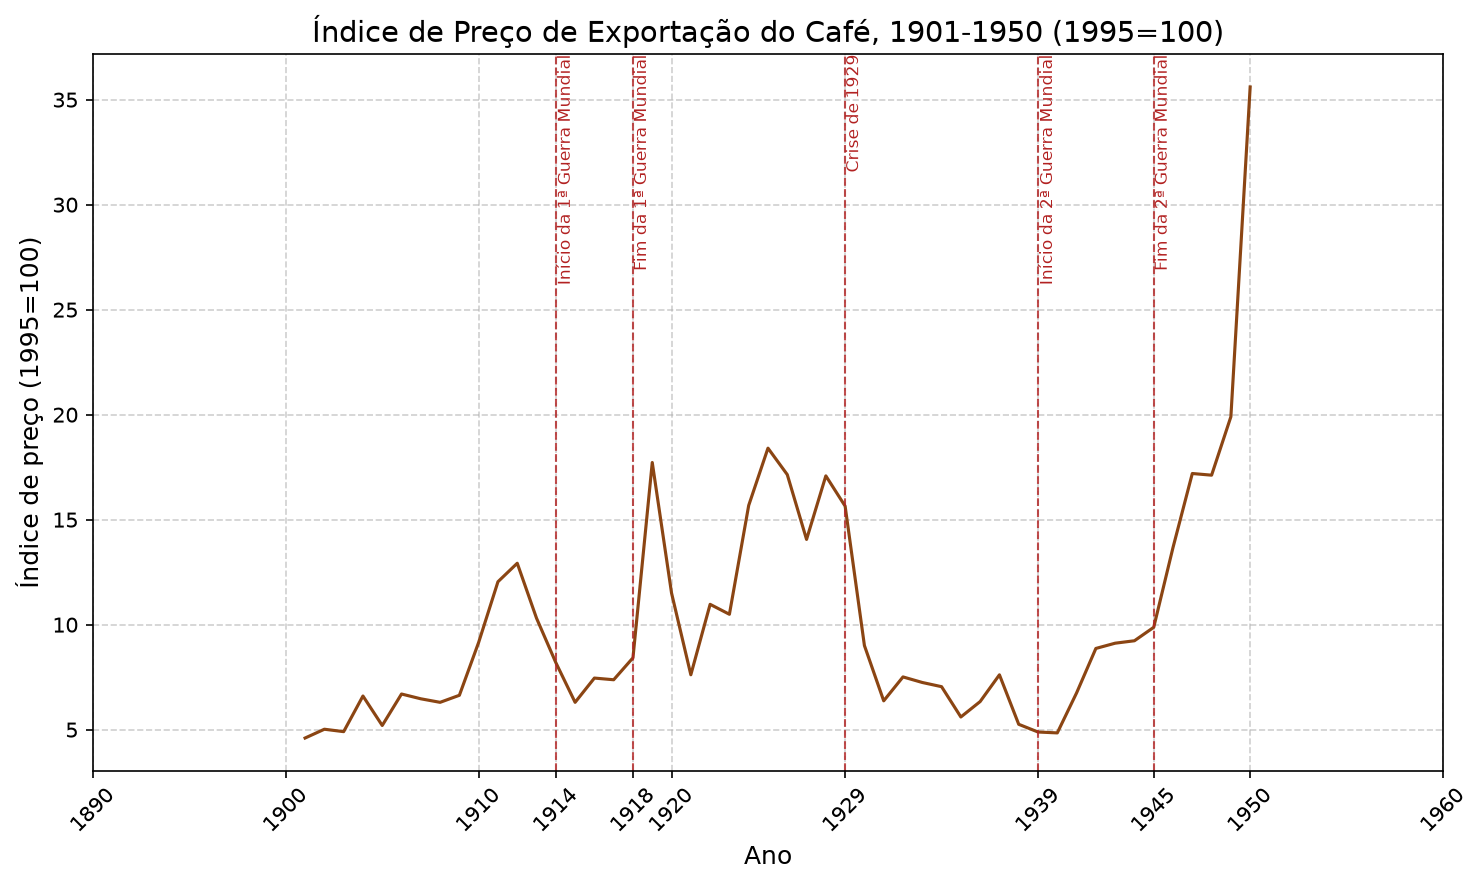
\includegraphics[width=\linewidth]{figures/cap04/preco_cafe_1901_1950.png}
\caption{Índice de preço do café, 1901--1950}
\label{fig:cap04-preco-cafe-1901-1950}
\aiflag{(fonte)}
\end{figure}

Da mesma forma, o impacto econômico derivado da desvalorização cambial
exerceu uma proteção ainda mais forte para os setores industriais
\citep{feijo_industrializacao_2023}, ao passo que também 
encareceu os custos da dívida contraída para
formação dos estoques de café. Se em outros momentos foi possível uma parcial
proteção do setor cafeeiro frente a quedas de preço, às vezes às custas
de outros setores da sociedade, via reajustamento entre preços externos
e internos via desvalorização cambial \citep{furtado2005}, 
a partir de 1929 tal dinâmica se mostra insustentável.

Isso não significa necessariamente uma mudança imediata dos rumos da política
econômica, entretanto. Elites orientadas a seus interesses de curto
prazo poderiam perfeitamente insistir na manutenção ou retomada da
priorização das atividades de seu interesse se devidamente bem
posicionadas para tal. Um impulso à indústria decorrente de um processo
relativamente espontâneo, entenda-se não intencionalmente coordenado
pelo Estado, de substituição de importações já havia ocorrido em função
da Primeira Guerra Mundial e larga medida já afetara profundamente a
trajetória industrial do país em relação ao período anterior \citep[]{suzigan2000}.
Mas a mudança da base econômica não foi, sozinha, capaz de alterar permanentemente a
política econômica. Da mesma forma, \citep[]{mello1982} aponta como ciclos de
acumulação financeira pelo setor cafeeiro, limitado em suas
possibilidades de expansão da produção, já estavam diretamente ligados à
acumulação produtiva na indústria. O que distingue o período posterior a
1929 de um mero choque externo, como antes, é que ele é também, em parte
justamente impulsionado pela crise, um momento de inflexão 
política. A saber, o golpe de 1930 e o início do período Vargas.

Não se pode evidentemente reduzir a revolução de 1930 ao choque
econômico da crise de 1929, apesar desta ter certamente contribuído. Ela
foi resultado de um conjunto de tensões e disputas, por exemplo, entre as
elites regionais, e de transformações graduais, como as dentro do
exército \citep[]{perissinotto_ideias_2023}. A base de sustentação inicial de Vargas certamente
continha aqueles favoráveis a projetos de industrialização ou
modernização da economia, como os Tenentistas \citep[]{schwarcz_brasil_2015},
mas estava longe
de ser uma revolução da burguesia industrial.

Pode-se observar essa dinâmica pelo seguinte fato:
se por um lado o apoio significativo do Estado aos cafeeiros,
especialmente os paulistas e as custas de outros setores, produz
insatisfação com o governo central antes de 1930, após a tomada de poder
serão feitos ajustes para oferecer estabilidade ao novo governo. A crise
de 1932, que culmina numa revolta paulista, é derrotada \citep[]{schwarcz_brasil_2015}, mas
logo em 1933 passam a ser tomadas significativas medidas de proteção ao
setor cafeeiro \citep{furtado2005}. Assim como em períodos anteriores, conflito e
conciliação se revezam e promovem grandes transformações graduais que
criarão as condições de mudanças ``abruptas''. Aqui destaca-se que o
forte impulso industrial só foi possível, pois havia um desenvolvimento
industrial prévio, particularmente após a primeira guerra, como aponta
Suzigan\citeyearpar[]{suzigan2000}. 
Furtado \citeyearpar[]{furtado2005} também pontua como a capacidade ociosa foi central
na possibilidade de se efetuar um primeiro ciclo de substituição de
importações mesmo diante de uma capacidade de importar bens de capital
limitada.

Tal discussão poderia sugerir que o desenvolvimento industrial
brasileiro não estava particularmente atrelado à conjuntura de 1930. Mas
ao contrário, é certo que não apenas a tomada de poder de Vargas
favoreceu as condições para o desenvolvimento industrial futuro 
\citep[]{perissinotto_ideias_2023}, através
de transformações institucionais importantes nessa primeira fase, como
sua manutenção no palácio do Catete foi em parte garantida por elas.
Apontam-se a seguir aspectos dessas transformações que apoiam tal
conclusão: a composição de classes e a(s) orientação(ões) ideológicas
desse governo; os impactos econômicos, intencionais ou não, de suas
políticas; as principais inovações relativas ao mercado de trabalho; as
inovações referentes ao planejamento econômico e o lugar dessa burguesia
industrial na coalizão varguista.

\subsection{O(s) governo(s) Vargas}

O período Vargas representou a ascensão de um novo
papel do Estado brasileiro em relação à economia. Tal postura não foi imediata 
e se operou em etapas graduais, concomitando
o processo de consolidação do poder político, o arranjo de classes
representado nas diferentes etapas do governo e graduais inovações
institucionais. Podemos separar o período no pós-golpe que vai de 1930
até 1934, marcado pelo conflito com a elite paulista cafeeira, da etapa
constitucional de 1934 até 1937 e do Estado Novo de 1937 até o fim da
segunda guerra em 1945 \citeyearpar{schwarcz_brasil_2015}. 
O período de 1930 até 1937 enfatiza
uma consolidação geral do poder e modernização do estado, com uma
significativa intensificação do desenvolvimentismo após 1937 \citep{perissinotto_ideias_2023}.

Quando olhada do ponto de vista das frações de classe, a aliança que trouxe Vargas ao poder
representava uma conjugação de forças tradicionais, particularmente as
classes ruralistas, com camadas emergentes das classes médias urbanas e
do exército. Ideologicamente havia um predomínio do pensamento
positivista, particularmente aquele oriundo do Rio Grande do Sul
\citep{perissinotto_ideias_2023}. Ao mesmo tempo, o tenentismo oferecia uma mistura de
positivismo já difundido no exército brasileiro
\citep{perissinotto_ideias_2023} com certo progressismo modernizante. Essa composição não
era estável, entretanto, com Vargas priorizando uma postura pragmática
\citep{schwarcz_brasil_2015} e despindo o positivismo de seus elementos mais
progressistas em prol daquele de perfil mais autoritário e tecnocrático, representativo
dos setores burocráticos civis e militares \citep{perissinotto_ideias_2023}. Com o tempo,
o próprio movimento tenentista acabou gradualmente sendo escanteado, em favor de
uma guinada integralista na estratégia de comunicação
Varguista \citep{schwarcz_brasil_2015} -- ela mesma que duraria apenas até o golpe de 1937 e
a tentativa de golpe integralista de 1938, que derrotada consolidava o
projeto de desenvolvimento positivista de Vargas.

Já principal oposição, a elite cafeeira de São Paulo, após conflitos
iniciais acabou parcialmente incorporada no governo, por ser 
ainda importante elemento para produção de divisas externas e
acumulação financeira. Mas a ``mentalidade industrializante''
\citep{perissinotto_ideias_2023} deste novo governo traria para o centro da dinâmica de
acumulação e do poder político brasileiro as elites industriais.

É importante notar, também, que havia uma participação mais
significativa das classes médias urbanas nesse projeto de governo,
associada tanto a pautas tenentistas como integralistas, que implicava
numa força política distinta a ser incorporada no projeto de país.
Assim, apesar de formalmente um rompimento com a ``república'', o
período varguista é marcado por uma incorporação crescente de setores da
sociedade, inclusive de operários e mulheres \citep{schwarcz_brasil_2015},
no projeto político, mesmo que tenha sido mantido uma clara orientação ``de cima
para baixo'' dessa transformação \todouser{}{Talvez citar Weffort aqui?} \aiflag{correção mecânica: faltava o segundo argumento obrigatório de \textbackslash todouser, o que faria o LaTeX engolir o próximo token (o ponto final) como descrição -- corrigido sem alterar o conteúdo.}.
Ao mesmo tempo, impulsionada pela
transformação econômica, essa nova composição entre frações de classe 
altera o projeto de país que emergia. Consumo das
classes médias urbanas, emprego industrial e um geral espírito de
modernização não poderiam ser obtidos por uma economia prioritariamente
agrícola e o desenvolvimento de um capitalismo industrial nacional
passava a ser imperativo par a manutenção do poder.

\begin{esboco}
\aiflag{[FIGURA A INSERIR: GRAFICO NUMERO DE TRABALHADORES NA INDUSTRIA]}
\end{esboco}

Do ponto de vista econômico, há que se fazer uma gradual diferenciação
do período. O crescimento industrial imediato e a tomada de poder em
1930 é significativamente mais restrito. Ele inicia um processo de
substituição de importações, ao qual Mello \citeyearpar{mello1982} entenderá como
ainda restrito e limitado às indústrias leves e àquelas voltadas a produtos de consumo.
Levará anos para a economia se recuperar de fato da crise de
1929, como para o novo governo consolidar seu poder político. Não à toa
a maioria das mudanças significativas operadas por Vargas se deram
após o golpe de 1937, também período que coincide com a aceleração do
desenvolvimento industrial brasileiro.

Ao mesmo tempo que estabeleceu boas relações com os industriais
brasileiros, Vargas também ocupou um papel de transformador das relações
de trabalho e angariou com isso significativo apoio da classe
trabalhadora \citep[]{schwarcz_brasil_2015}. Um conjunto de reformas institucionais
reorganizou o mercado de trabalho nacional, dando tanto ganhos às
classes trabalhadoras como permitindo a gestão do conflito trabalho
capital pelo Estado. Assim como na imigração para o café paulista, o
papel do Estado como mediador das relações trabalhistas se mostrou
necessário para permitir a adoção de padrões de trabalho acima do que as
elites econômicas estavam inicialmente dispostas. Exemplifica assim um
caso em que os dispositivos de mercado não necessariamente operam
adequadamente apenas com base em relações de oferta e demanda. A
construção consciente e estatal de certos padrões para o mercado de
trabalho foi necessária para garantir a reprodução do capital
industrial, assim como tinha sido para a expansão do capital cafeeiro.

\begin{esboco}
\aiflag{[FIGURA A INSERIR: GRAFICO GASTOS DO ESTADO]}
\end{esboco}

Sobre tal capital industrial, este continuava a crescer associado às
atividades exportadoras. Entretanto, cada vez mais se aproveitava de
espaços abertos na estrutura burocrática, além de reforçar suas
entidades de classe \todouser{}{identificar citação correta}.
As transformações entre fim do século XIX e
primeiras décadas do XX já tinham dado força à burguesia industrial --
que já se organizava desde 1827 em organizações como a Sociedade
Auxiliadora da Indústria Nacional. Esta passou a ser capaz de defender
seus interesses, não sendo mera subsidiária do setor exportador
\citep[]{perissinotto_ideias_2023}

Essa fração de classe não era, entretanto, homogênea. Sua própria origem
enquanto capital nacional já remetia tanto a grandes senhores de terras
buscando diversificar sua atividade econômica, mas também uma
significativa origem nas populações imigrantes \citep[]{jr_historia_2021}.
Enquanto capital estrangeiro, diferenciava-se pelos setores importadores e exportadores
associados à atividade industrial, pelos investidores em infraestrutura,
pelas indústrias maquiladoras e pelo capital financeiro, financiador de
atividades privadas e do Estado \citep[]{jr_historia_2021}.
Este último segmento do capital parece
se mostrar o mais hegemônico \citep[]{jr_historia_2021} e consolidar um modelo de
extração de rendas, via reenvio de lucros, de pagamentos de juros
de empréstimos ou da dívida pública brasileira, que será importante
parte do porquê a industrialização brasileira se consolidou como
dependente nas décadas seguintes \citep[]{evans_dependent_1979}.

Uma distinção para os processos de outros países previamente
industrializados foi que a industrialização brasileira não ocorreu, do
ponto de vista da técnica, de forma gradual e sim pela superimposição de
``unidades tecnológicas modernas'' {[}...{]} `` para atender uma demanda
preexistente'' (Candall, 2009 \emph{apud} \citeauthor{feijo_industrializacao_2023},
\citeyear{feijo_industrializacao_2023}). Esse processo é justamente fruto da
industrialização tardia, que associa a característica do processo
de importação a estrutura dual do mercado de trabalho e sociedade . \aiflag{repetição de palavra: ``processo'' aparece duas vezes nesta mesma frase e mais duas vezes no entorno próximo (parágrafos acima e abaixo, ex. ``processo de industrialização''); considerar variar com ``dinâmica'', ``mecanismo'' ou ``trajetória'' em uma das ocorrências.}

Tal condição cria padrões de substituição de importação não orientados ao
atendimento das necessidades e demandas da maior parte da população,
excluída do consumo, mas prioritariamente de uma elite. Tal cenário se
dá mesmo com relativo crescimento do setor assalariado, em parte
impulsionado justamente pela indústria. Prado Jr. \citeyearpar[]{jr_historia_2021}
enfatiza a diferença de uma indústria desenvolvida num país \emph{produtor,} por virtude do
passado colonial, e não \emph{consumidor}. Assim a indústria se
desenvolve fora de estágios ou necessidades graduais e apenas para
satisfazer demandas de consumo muito especializadas, causando ausência
de continuidade -- técnica -- no processo de industrialização. Como
veremos mais adiante, também implica em ciclos recorrentes de
estrangulamento cambial devido aos novos setores ``nacionalizados''
ainda requererem significativas importações \cite{tavares1973}.

\begin{esboco}
\aiflag{[FIGURA A INSERIR: GRAFICO TIPOS DE INDUSTRIA DE transformação]}
\end{esboco}

De toda maneira, a indústria passa a ser o principal explicador do
desempenho da economia, em lugar da agricultura. Internamente o
dinamismo reflete a mudança da estrutura da atividade industrial, com
maior peso a setores mais dinâmicos. Realiza-se, portanto, uma
transferência de mão de obra, capital e tecnologia para setores mais
produtivos \citep{feijo_industrializacao_2023}. Mas nossa industrialização dependeu também da
marginalização de grande parte da população e do desemprego disfarçado,
ao se basear num câmbio desnivelado, em inflação e baixos salários
\citep{pradojunior2012}. Além disso, a posição privilegiada do
capital estrangeiro o permitiu tomar proveito desse processo de substituição de
importações, via implementação da produção parcial ou integral no país \citep{pradojunior2012}.
Elas ocuparão assim os núcleos mais dinâmicos da industrialização -- o que
Evans \citeyearpar{evans_dependent_1979} argumenta será intensificado nas décadas
de 1960 e 1970 --  como, por exemplo, o automotivo,
tanto via esse processo como via financiamento e
empréstimos decorrentes do desequilíbrio nas contas
externas.

Assim, o capital estrangeiro assume uma parcela cada vez mais
privilegiada da economia brasileira \citep{pradojunior2012}, estabelecendo relações de
interesse mútuo e de segmentação de setores com
às elites industriais nacionais e o capital estatal, o que em última instância
produz aquilo que Evans\citep{evans_dependent_1979} 
denominou uma ``Tripla Aliança'' nos anos 1970 -- setores de
alto crescimento com predomínio de capital estrangeiro, setores
estratégicos e de alto risco associados ao Estado e setores de bens de
consumo menos sofisticados para o capital nacional privado.

É preciso reforçar novamente que a revolução de 1930 não foi uma tomada de poder
pelos industrialistas, estes estiveram na margem desta apenas.
Mas a orientação positivista do novo governo \citep{perissinotto_ideias_2023} e dos
militares implicava na necessidade de um desenvolvimento
industrial. Assim como a elite rural foi catapultada pela vinda da
família real e depois pela independência como portadora de um projeto de
país, a elite industrial foi alçada à posição de ponta de lança do novo
modelo de desenvolvimento. Instrumentalmente, sua influência foi gradual
e a reboque de forças políticas mais consolidadas. Estruturalmente, ela
passou a ser a fração de classe que guiava o crescimento econômico
brasileiro.

Vargas foi assim a primeira experiência de planejamento econômico por
parte do Estado brasileiro \citet[]{kon_quatro_1994}\todouser{}{Aidionar Suzigan tb}, ao mesmo tempo que vai consolidar o
modelo de acumulação centrado na indústria. Até então a preocupação era
centrada na preservação das atividades econômicas dominantes,
particularmente os setores primários exportadores, em muito orientada
também pela necessidade de financiamento do aparelho público. Em Vargas
vê-se pela primeira vez um esforço de transformação da estrutura
econômica, da composição de atividades econômicas do país, a partir da
perspectiva de que dadas atividades, em particular àquelas orientadas à
indústria, eram de importância estratégica.

Os primeiros planos eram orientados a suprir carências de
infraestrutura, educação, segurança alimentar e indústrias de base
\citet[]{kon_quatro_1994}. Conjugavam assim pautas desenvolvimentistas com melhorias ao
padrão de vida e consumo da população. Não eram projetos redistributivos
ou que atacassem diretamente a desigualdade econômica, mas pela primeira
vez emergia uma concepção de ``desenvolvimento'' onde o bem-estar social
precisava estar associado ao crescimento das atividades-chave, mesmo que
ideologicamente funcionando como uma espécie de seguro anticomunismo. Essa
incorporação de algum grau de pressão popular sobre a elite política será
chave para entendimento da política brasileira até 1964 \citep[]{weffortPopulismoNaPolitica2003}.

Para além da transformação política, o contexto econômico dos anos 1930
ampliou a capacidade de desenvolvimento da indústria. Ao longo da década, praticamente todas as
economias latino americanas abandonaram de fato a tentativa de
preservação do padrão ouro \citep{bethell_cambridge_2009,bethell_cambridge_2009-1}. Como consequência, uma
forte desvalorização cambial se deu, operando significativo fator
protetor às nascentes indústrias nacionais.

No que se refere ao comércio externo, a década de 30 é marcada pela
deterioração dos termos de troca e pela queda nas exportações. Havia
segmentação e monopólio da taxa de câmbio pelo Banco do Brasil, que
recebia a receita total das exportações e também o controle seletivo das
importações por orientação do governo \citep{feijo_industrializacao_2023}.
Feijó \emph{et al} ~\citeyearpar[]{feijo_industrializacao_2023}
concluem daí que período teria sido fortemente intervencionista, em contraste
com anos 1920. Além disso, a limitação das importações,
por efeito das quedas das exportações de café (ver Figura~\ref{fig:cap04-preco-cafe-1901-1950}), permitiu avanço da
indústria de substituição. Em conjunto operou a política de sustentação
do preço do café, que contribuiu a pela sustentação da demanda agregada.

O fim do padrão ouro não marca, entretanto, o fim da dependência
externa. Na verdade, em meio ao processo de substituição de importações
significativo papel acabou sendo dado às indústrias maquiladoras, que
nacionalizaram as etapas de montagem de seus produtos como forma de
acesso ao mercado nacional \citep{pradojunior2012}. Esse modelo de
investimento industrial externo visando acesso ao mercado nacional será em parte
preservado até os dias atuais. Aliás, a relação entre uma postura
nacionalista e o apelo ao capital estrangeiro sempre foi uma dubiedade
de Vargas, com ambas as correntes de pensamento representadas em seu
governo \todouser{}{Citar Fausto}.

\todouser{}{GRÁFICO COMERCIO EXTERNO E DIVIDA EXTERNA}
\aiflag{A parte da dívida externa já está ilustrada na Figura~\ref{fig:cap04-divida-externa} (não duplicada aqui). Falta apenas o gráfico de comércio externo -- dado já disponível em tables/cap04/exportacoes\_importacoes/externo\_1900\_1939.csv ou externo\_1900\_2000.csv, sem imagem produzida.}

Retomando, a vitória de Vargas no conflito com os paulistas é seguida de uma parcial
repactuação de forças com o período constitucional de 1934 \citep[]{schwarcz_brasil_2015}.
Um dos mais importantes sinais dessa dinâmica é citado conjunto de medidas protetivas ao
café erguido por Vargas. Ao passo que se impunham um conjunto de
interventores nos governos estaduais e tentava-se limitar a capacidade
de reação das elites locais, também era preservado o mecanismo de
acumulação cafeeiro \citep[]{mello1982}. Como em diversos momentos da história
anterior, a ampliação da capacidade de exportação de produtos primários
era importante elemento na arrecadação do governo e também na entrada de
divisas que permitiam importação necessária às novas atividades
industriais \citep[]{mello1982,tavares1973}.

O que muda é que, a partir de 1934, mesmo diante da melhora de preços
fica clara a incapacidade de um ciclo de acumulação continuar baseado na
exportação. Também ficam consolidados no poder representantes de
diversos interesses que não podiam ser atendidos pela dinâmica de
acumulação do café, borracha, açúcar ou qualquer outro produto primário
exportador.

\begin{esboco}
\aiflag{[FIGURA A INSERIR: GRAFICO GASTOS DO ESTADO]}
\end{esboco}

O fim dos anos 1930 e a emergência da Segunda Guerra Mundial em 1938 vão
estressar internamente o novo governo por sua dubiedade a respeito tanto do
papel do capital estrangeiro, como de seu alinhamento político e
ideológico frente aos conflitos emergentes no centro do capitalismo. Há
discussões sobre a maior proximidade ideológica de Vargas com o fascismo
italiano, mas também há considerações sobre seu caráter pragmático e
desconfiança dos movimentos fascistas nacionais \citep[]{schwarcz_brasil_2015}. O que parece
claro é que Vargas, e a estrutura burocrática do governo e exército,
viam com desconfiança qualquer força de massas que pudesse se tornar
opositora de seu projeto. Perissinoto \citeyearpar[]{perissinotto_ideias_2023} argumenta que um
positivismo de caráter autoritário seria uma definição mais precisa do projeto
que se consolida do que o integralismo ou fascismo estritamente falando.

Para o autor, o período continha duas alternativas claras, positivismo
com protecionismo industrialista -- que dará origem ao
desenvolvimentismo cepalino -- e o integralismo. Protecionismo foi a
escolha da ``nova elite no poder'' que o via como questão de interesse
nacional e parte da busca de independência econômica e soberania
política \citep{perissinotto_ideias_2023}. Gradualmente sua influência cresceu ao longo da
história brasileira, se tornando hegemônico, enquanto o integralismo foi
derrotado em 1938, após tentativa de contra golpe ao Estado Novo (1937)
e desaparecerá até 1945 \citep{perissinotto_ideias_2023}.

O positivismo desenvolvimentista desde então será base ideológica do
processo de industrialização, orientado por uma nova elite advinda da
burguesia industrial, que buscava oportunidades pragmáticas de
obter representação no Estado e interferir na política econômica. 
Este é particularmente um positivismo orientado à ação
prática. Perissinotto \citeyearpar[]{perissinotto_ideias_2023}
atribui essa trajetória às ideias econômicas do positivismo riograndense
e castilhista, cuja elite será central no período pós 1930,
a começar pelo próprio Vargas. Esse Sul
castilhista foi terreno fértil para um positivismo mais político e
atuante/prático, orientado à formulação de políticas públicas e
construção de instituições -- contrastando com aquele religioso e o
intelectual \citeyearpar[]{perissinotto_ideias_2023}.
Também defendia a ocupação de cargos públicos e acelerar a
transformação da sociedade, o que ajudava a constituir uma burocracia
ativa no processo de desenvolvimento \citep[]{bresser-pereira_burocracia_2007}.

É importante também entender o positivismo por sua característica como
uma ideologia de classe média com força em meios civis e militares e
escolas de formação técnica. Estes buscam uma
organização do mercado caótico via Estado, racionalizado e autoritário,
com defesa de uma cultura técnico-científica e da educação laica e
profissionalizante \citep{perissinotto_ideias_2023}. Os positivistas se percebiam como
modernizadores da sociedade e apoiavam um estado centralizado e
controlado por elite técnica a serviço da industrialização. De fato,
foram pioneiros em defender a modernização de um país de terceiro mundo,
antes mesmo da ascensão da CEPAL, que advém do período pós-Segunda Guerra Mundial
e dos movimentos de libertação nacional \citep{perissinotto_ideias_2023}. Também se
contrapõe a uma tradição bacharelesca e aristocrática, que tinha
permanecido do Império e ao longo da primeira república \citep{perissinotto_ideias_2023}.
Era, assim, sinal de incorporação do pensamento e interesse novos grupos
sociais no processo de desenvolvimento, mas efetuado por elites
conservadoras e tendo como principais beneficiários elites industriais,
parcialmente produtos da antiga elite cafeeira. Opera-se assim um
processo de transformação ideológica que implementa um projeto de país
tão disruptivo em suas ideias, instituições e organizações, quanto
conservador em suas classes dominantes e estrutura social.

Outro ponto onde o governo Vargas tinha uma posição dúbia
era a respeito do papel do capital internacional,
o qual era visto com entusiasmo por alguns, como
necessário por outros e como danoso à soberania pelos demais
\citep{perissinotto_ideias_2023}.
De forma pragmática, Vargas manteve o
máximo que pode essa dubiedade, abrigando em seu governo representantes
mais e menos afeitos ao capital estrangeiro. Porém, uma definição mais
clara de sua posição começa a se tornar crítica na emergência da Segunda Guerra Mundial.
O conflito situado no centro do capitalismo
obrigava o governo brasileiro a escolher um lado, por assim dizer, ao
mesmo tempo que internamente debatia as virtudes do capital estrangeiro
como um aliado ao desenvolvimento nacional ou uma ameaça à verdadeira
soberania \citep{perissinotto_ideias_2023}. 
A atuação do governo americano, com força
de seu domínio tecnológico e financeiro, junto às conjunturas políticas locais
-- inclusive o afastamento do integralismo -- e a necessidade prática de
investimentos em setores-chave definiram por parte do governo uma guinada pró EUA e maior
abertura econômica.

A partir da década de 1940, portanto, toma corpo e acaba por vencer a
posição mais favorável ao capital estrangeiro. Mais do que
apenas a mudança de influência ou a escolha ideológica, o movimento é
significativo de uma transformação no \emph{locus} global da acumulação
de capital, que justamente se consolida na segunda guerra e arrasta o
Brasil para sua semiperiferia \citep{wallerstein2001,arrighiseculoxx}. Se anteriormente
a economia nacional já tinha transitado de uma relação de dependência
com o modelo de acumulação holandês para o inglês, agora transitava para
um novo modelo de acumulação do capital centrado nos EUA \citep{arrighiseculoxx}.

Talvez o maior símbolo interno dessa mudança tenha sido a implementação
da Companhia Siderúrgica Nacional (CSN) com capital americano. \aiflag{sugestão de citação: este parágrafo sobre a CSN e o financiamento americano não tem nenhuma citação de apoio -- vale reforçar com uma fonte específica sobre a fundação da CSN.} Esta,
apesar de só efetivamente começar a operar após a guerra, representava o
protagonismo estadunidense no desenvolvimento da economia brasileira, ao
mesmo tempo que auxiliava o desenvolvimento de um setor estratégico para
Vargas. Era assim símbolo de uma espécie de nacionalismo pró
norte-americano que substituiu nosso liberalismo unilateral pró
Inglaterra. As consequências dessa transformação irão não apenas
atravessar as décadas seguintes, como ainda hoje se repercutem numa
posição onde grupos políticos de discurso nacionalista-conservador
operam alinhamento automático de sua concepção de desenvolvimento
nacional ao interesse dos EUA. Muito antes, entretanto, será
determinante para escolhas políticas e desenvolvimentos econômicos que
comandarão a industrialização brasileira após a queda de Vargas.

Caminhando para as demais transformações do governo Vargas, podemos
esquematicamente separar -- a partir do levantamento de Cano \citeyearpar[]{canocintra1974}
 -- entre: 1-criação de organizações, 2-planos e programas,
3-órgãos de coordenação, instituições de financiamento. Além destes
houve a implementação de diversas normas gerais a respeito da política
econômica, tributária e cambial e das políticas migratórias, sindical e
trabalhista. A ênfase aqui será nos três itens numerados, que mais diretamente
refletem as estratégias de planejamento econômico do Estado no período.

Do ponto de vista das estatais e organizações, as responsáveis pelo maior volume de investimentos 
na política de industrialização pelo setor
público, temos a abertura da já citada CSN em
1941, do Departamento Nacional de Estradas de Ferro (1941), da Fábrica
Nacional de Motores em 1941 (com liberação de crédito já em 1941), da
Companhia hidrelétrica do São Francisco em 1943 (mas que iria funcionar
apenas em 1955) e da Cia Vale do Rio Doce em 1942, esta última
explicitamente criada como uma tentativa de manutenção do controle
nacional no setor de mineração \citep{canocintra1974}.

Essa oscilação entre maior abertura ao capital estrangeiro ou
nacionalismo econômico, que se reflete de forma clara na distinção entre
a CSN e a Vale do Rio Doce, é um reconhecimento da
condição de dependência econômica, mas com postura pragmática para
solucioná-la. Havia assim, clareza de que o uso do capital estrangeiro implicava
uma condição distinta do capital nacional na atividade industrial. Aqui,
entretanto, ainda não parecia haver uma clareza total de quais áreas
deveriam ser abertas ao capital estrangeiro ou fechadas, sua escolha
refletindo mais as conjunturas internas do governo. Ao longo dos
governos seguintes será cada vez mais clara a posição -- às vezes
privilegiada -- do capital estrangeiro e a reserva de espaços para o
capital nacional, além de particular posicionamento do capital estatal
em setores ``estratégicos'', como discutido por Evans \citeyearpar{evans_dependent_1979}.

Do ponto de vista do planejamento econômico destacam-se tanto o plano de
obras públicas e de defesa nacional (1931) como o Plano de Obras e
Equipamentos (regulamentado em 1943, implementado de 1944 até 1948).
Ambos tinham como finalidade parcial o
desenvolvimento de indústrias básicas \citep{canocintra1974}, o que já
denota um esforço consciente de mudança em relação ao modelo de
substituição de importações anterior.

Entre os diversos institutos e órgãos estão também do Instituto do
Açúcar e Álcool (1933), o Instituto de Tecnologia, até 1933 vinculado ao
ministério da agricultura e a partir de 1934 ao ministério do trabalho,
a criação de carteiras de crédito agrícola e industrial (1937), do
Conselho Nacional do Petróleo (1938), de Águas e Energia elétrica (1939)
e a comissão executiva do plano siderúrgico nacional (1940). É
importante também notar como a transição ao longo dos anos 1930 abarca
uma redução gradual da dependência do setor agropecuário como
justificativa ou motor principal da política pública e crescente
protagonismo do setor industrial.

Já no que tange a regulação do trabalho, a transformação institucional de maior relevância foi a
Consolidação das Leis Trabalhistas, em 1943 \citep{feijo_industrializacao_2023}. Na verdade,
ela marca o auge de uma relação aonde parte importante da sustentação de
Vargas será dado pelo apoio de trabalhadores, via uma direta interferência do
Estado no mercado de trabalho e relações sindicais que, ao mesmo tempo,
promovia ganhos e direitos aos trabalhadores. Constitui-se ali a participação de massas
como elemento de pressão política, no que Weffort \citeyearpar{weffortPopulismoNaPolitica2003}
denominará populismo -- sem ali os mesmos contornos normativos que a terminologia recebe
em tempos atuais.

Num olhar mais amplo, governo Varguista estabeleceu bases da legislação trabalhista, sindical e
previdenciária, mas manteve sobre eles significativo controle,
acalmando temores de comunismo por parte do empresariado \citep[]{schwarcz_brasil_2015}
A aplicação dessa legislação especificamente ao trabalhador urbano,
demonstra tanto como o trabalhador industrial era central e visto com mais
capacidade de organização e força política que outras camadas sociais ou
os próprios trabalhadores rurais -- que ficaram excluídos da CLT -- como a capacidade
das elites agrárias de preservarem instituições que lhes permitissem conservar relativa
capacidade de acumulação.

Vargas propunha assim uma via de inserção conservadora para grande parte da mão
de obra urbana que tinha sido relegada em função da estrutura econômica
centrada na exportação de commodities agrárias, algo apenas possível via
a estrutura dual da sociedade se refletir também numa divisão
rural-urbano significativa, como apontado por Prado Jr. \citep{pradojunior2012}.

Assim, especialmente após 1937, o governo Vargas estabeleceu as bases
institucionais do planejamento econômico brasileiro, especialmente no
que concerne à infraestrutura e à indústria de base. Havia pouco avanço
no sentido da elaboração de artigos de consumo mais sofisticados, mas já
revelava uma preocupação com pontos nevrálgicos da infraestrutura
brasileira que se repetiria no futuro, tanto no segundo governo Vargas,
como no governo JK e na ditadura militar.

O primeiro governo Vargas se encerra em 1945. Em geral, historiadores
associam sua saída do poder a demandas populares por democracia após o
fim da Segunda Guerra Mundial, especialmente internas ao exército
\citep[]{schwarcz_brasil_2015}. É fato de que, se a democracia estava em descrédito nos anos
1930, esta assume grande valor simbólico após 1945. Curiosamente, é
justamente um conjunto de transformações ocorridas durante o regime
varguista, como o direito de voto a mulheres -- reconhecido em 1932 e
presente na constituição de 1934 --, que permite a esse posterior
período democrático oferecer uma participação popular mais significativa
do que a república anterior.

O retorno à alternância de poder também marcará uma retomada de maior
inconstância na política econômica. Mesmo assim, até mesmo governos de
viés liberal acabarão adotando parte significativa do repertório
desenvolvimentista, o primeiro deles sendo o governo Dutra.

Também se manterá, ao menos até 1964, uma maior capacidade de pressão das
classes trabalhadoras, além de maior inclusão no processo político
-- ou ao menos consideração por este -- de classes médias e
diversos grupos sociais na sociedade. Isso mostra, de forma contraintuitiva ao
caráter autoritário e mesmo ditatorial, que o período Vargas foi
importante construtor institucional de uma maior participação popular
que será influência importante de 1945 até 1964, promovendo o que
Barbosa \citep{barbosa_developmentalist_2020} vai denominar como um breve período de um
desenvolvimentismo democrático no Brasil. Nesse período, o modelo de
desenvolvimento ancorado na industrialização não apenas é preservado
quantitativamente -- crescimento da indústria e sua participação na
economia --, mas terá avanços qualitativos quanto à natureza da
atividade industrial promovida.

\section{1945-1964: redemocratização e dívida}\label{redemocratizauxe7uxe3o-e-duxedvida}

Como discutido, a partir da década de 1940 o Brasil passou a consolidar
uma nova relação de dependência, agora primariamente vinculada aos EUA. Apesar dessa
aproximação ocorrer em meio ao governo Vargas, a associação deste com o
nacionalismo de inspiração fascista e a propagação de um modelo
democrático liberal como forma vencedora do conflito levaram a sua
queda. Contribuíram para isso tanto a pressão americana \todouser{}{inserir FAUSTO}
\aiflag{correção mecânica: faltava o segundo argumento de \textbackslash todouser (o LaTeX engoliria a letra seguinte do texto como descrição) -- corrigido sem alterar o conteúdo.}
como as condições internas, sejam elas interpretadas como anseios
democráticos \citep{schwarcz_brasil_2015} ou como reorientação de interesses de frações de
classe. Também se colocava um contraste entre uma política nacionalista,
com claro uso do elemento cambial como forma de proteção e estímulo a
indústria, e os parâmetros estabelecidos em Bretton Woods em 1944 \aiflag{sugestão de citação: a menção a Bretton Woods e seus parâmetros está sem fonte -- considerar uma referência sobre o sistema de Bretton Woods e sua relação com a política cambial brasileira.}. Além
disso, é fato que em 1945 a economia já enfrentava um crescente problema
inflacionário e também de balanço de pagamentos \todouser{}{Referenciar BP} e
a simpatia do exército a causa permitiu aos opositores de Vargas sua
derrubada.

Seu sucessor, o governo Dutra, parecia contar com um conjunto de premissas
sobre o cenário econômico e geopolíticas, diga-se: substanciais reservas internas, apoio
americano, crescimento do livre comércio e, fruto das duas últimas,
entrada de dólares \citep{vianna_o_2025}. O receituário foi, portanto a
adoção de um livre comércio de câmbio \footnote{\todouser{}{NOTA DO AUTOR: Diferenciar livre
'comércio de câmbio' de 'câmbio flutuante'}} e de um ajuste ortodoxo,
reduzindo despesas em prol de conter a inflação \todouser{}{Pegar dados despesas públicas}.

Os esforços, entretanto foram mal sucedidos. Ao contrário do esperado, o
pós-Segunda Guerra Mundial foi caracterizado por uma escassez de
dólares. Em particular, prejudicou o governo a lenta adoção do
padrão-dólar pelas demais nações. Em poucas palavras, o Brasil acumulava
divisas em moedas de diversos países, mas estas não eram imediatamente
convertíveis em dólar. A piorar, as vendas de café, ainda importante
produto de exportação, eram destinadas a um conjunto diverso de países o
que, na prática, significava que mesmo um saldo comercial positivo não
se refletia proporcionalmente na entrada de divisas conversíveis \citep[]{vianna_o_2025}.

Como em diversos outros momentos anteriores e futuros de nossa história,
a conjuntura forçou então uma mudança pragmática na atuação do governo.
O governo passou a adotar um padrão mais intervencionista, eliminando o
livre comércio e implementando gradualmente um controle de importações
entre 1947 e 1948 baseado em licenças de importação \citep[]{vianna_o_2025}.

Combinou-se assim um câmbio sobrevalorizado -- que facilitava importação
de matérias-primas e bens de capital -- com uma restrição de importações
-- que restringia a competição estrangeira. Tal combinação teve como
efeito um significativo processo de substituição de importações que
manteve o crescimento industrial mesmo em meio a política de austeridade
\citep{vianna_o_2025}. Evitar a desvalorização cambial não era a princípio
um mecanismo de industrialização, mas serviu muito bem como. O resultado
desse aprendizado será sua adoção regular em futuros governos.
Adicionalmente, contava com uma política de expansão creditícia do Banco
do Brasil \citep{vianna_o_2025}.

Ao fim, de fato foi obtida redução do déficit em moeda controlada e
inicialmente uma baixa da inflação, que gradualmente subiu novamente e
passou a ter aceleração significativa em 1949, frente a mudança no
ministério da Fazenda e expansão de gastos visando as eleições \citep[]{vianna_o_2025}. 
Do ponto de vista do investimento público, esse não foi tão
significativo na expansão industrial, a exceção da finalização da
construção da CSN. O próprio plano SALTE pouco efeito teve diante a
ausência de mecanismos de financiamento \citep[]{vianna_o_2025}, apesar de ter previsto
inovações futuras relevantes como a criação de um banco de
desenvolvimento -- futuro BNDE.

Entreposto dos dois Governos Vargas, o período Dutra costuma parecer
menos transformativo do quadro geral da economia brasileira, mas essa
aparência esconde não apenas um forte crescimento industrial, mas também
uma representatividade da dinâmica de governos e políticas econômicas
durante quase todo o século XX. Primeiro, os ``vilões'' típicos estão
ali, uma inflação forte e uma crise cambial. A resposta a primeira, uma
tentativa de contenção de gastos total ou parcialmente frustrada já fora
feita anteriormente e será repetida no início do próximo governo Vargas,
dos governos Jânio e Castelo Branco e em momentos posteriores. Segundo,
o impacto do condicionamento da economia brasileira à política
norte-americana, intermediado por uma expectativa de alinhamento quase
sempre unilateral. Para além desses fatores, criou um dos mais
importantes mecanismos de promoção da substituição de importações, o
controle de importações via sistema de licença. Este representa uma
recorrência, instituições que surgem e evoluem não de planejamentos
conscientes, mas do aprendizado sobre efeitos inesperados de políticas
anteriores.

O período também ressalta como a conjuntura direciona as elites a um pragmatismo
político. As inclinações ideológicas dos governos são indicadores, mas
não determinantes da sua efetiva atuação. Um dos fatores que impõe isso
é a continuidade de um núcleo burocrático ideologicamente orientado a um
projeto de desenvolvimento industrializante e que pôde em parte resistir
ao direcionamento do governo da época \citep{perissinotto_ideias_2023,bresser-pereira_burocracia_2007}. 
O outro elemento é a transformação das forças relativas entre as
frações das classes dominantes. Aqui o grande grupo em ascensão é a
classe industrial, o que explica a existência da
contradição entre uma política de austeridade no ministério da Fazenda e
uma política de expansão de crédito no Banco do Brasil,
mais próximo da esfera de influências dos industrialistas.

A força dessa classe burguesa é acompanhada de um fortalecimento de
diversos setores das classes trabalhadoras, tanto daqueles operários
industriais como de setores da classe média afáveis a um projeto
político que colocasse a indústria na centralidade do desenvolvimento
econômico. É nesse contexto que Vargas vence a eleição de 1950 pelo PTB,
defendendo a industrialização e também a ampliação da legislação
trabalhista \citep{vianna_o_2025}. A instabilidade política voltava a se
refletir nos questionamentos dos setores derrotados à legitimidade das
eleições, mas o apoio de setores das forças armadas à legitimidade do
processo fez prevalecer a eleição \citep{fico_historia_2022}.

O segundo governo Vargas é um marco importante, visto que
representa o ponto de partida de importantes transformações internas ao
Estado, mas também de um novo contexto de mudanças sociais na sociedade
brasileira e no mundo ao longo da década de 1950. Do ponto de vista
internacional é a década de acirramento de tensões geopolíticas da
Guerra Fria. A oposição entre o modelo americano, hegemônico
após a Segunda Guerra Mundial, de um lado, e o modelo soviético de
outro. Em alguns casos, como na
Europa Ocidental e Leste Asiático, o efeito dessa disputa é um maciço volume de
investimentos americanos. Do ponto de vista do trabalho, é uma década de
fortalecimento dos sindicatos nos EUA e do estabelecimento do modelo de
bem-estar social na Europa Ocidental, que também começa a exibir os
primeiros sinais de um processo de desindustrialização \todouser{}{citar fonte}.

Esses efeitos são modulados na América Latina, primeiramente por essa
aparecer como menos prioritária nos esforços anti socialista americanos.
Isso reflete num menor grau de apoio, mesmo que este ainda exista,
comparado a outros casos. Como consequência, boa parte dos investimentos
americanos e europeus no Brasil no período serão de caráter privado,
orientados por interesses de ocupação de mercados privilegiados. Isso
implica que os governos precisarão oferecer maiores atrativos,
comparativamente, a este capital ou impor maiores restrições às
importações.

Do ponto de vista interno, é uma década de intensa urbanização e
crescimento populacional, com particular concentração no Sudeste. Como
consequência é uma década marcada por ondas significativas de
trabalhadores Nordestinos para o Sudeste \citep[]{fontes_migration_2016},
contribuindo para um processo de crescimento desordenado das grandes capitais, além de
significativos impactos econômicos para o Nordeste decorrentes da saída
da mão de obra produtiva. É nesse cenário que vai se consolidando ainda
mais uma classe trabalhadora urbana, e boa parte proletária, que
passa a ser significativo ponto de apoio de linhagens políticas que, em
maior ou menor grau, vão se identificar com um certo ``Getulismo''
\todouser{}{Citar getulismo} ou mais amplamente uma ideia de ``Trabalhismo'' \todouser{}{Citas trabalhismo} \aiflag{correção mecânica: as duas ocorrências de \textbackslash todouser acima estavam com apenas um argumento, o que faria o LaTeX engolir o token seguinte (uma letra e o ponto final, respectivamente) como descrição -- corrigido sem alterar o conteúdo ou a grafia original das notas.}.
Será nessa aliança entre setores nacionalistas e desenvolvimentistas da elite
política, setores industriais da elite econômica, uma parte mais
desenvolvimentista do exército e setores operários urbanos da classe
trabalhadora, que se consolidará a maior força política do país até o
golpe de 1964. Em contraponto a esta aliança estará fundamentalmente uma
elite política conservadora, aliada a setores liberais ou ruralistas da
elite econômica, setores mais conservadores e anticomunistas do exército
e camadas populares mais conservadoras.

O segundo governo Getúlio é uma síntese desse embate, sendo eleito ao
fim de um projeto liberal mal sucedido ele conterá constantes conflitos,
com particular ênfase as questões trabalhistas, que culminarão na
tentativa de deposição em 1954 e em seu suicídio, que pode ser
considerado peça fundamental no adiamento de um possível golpe de Estado
para 1964. Antes de avançar, entretanto, é preciso descrever o conjunto
de políticas chave e o contexto econômico que acirraram tal disputa.

O período entre 1945 e 1950 exibiu forte crescimento econômico
e industrial, mas abaixo do que se observou nos períodos seguintes.
Também manteve a trajetória típica de uma tentativa inicial de atração
de capitais e ajuste fiscal para controle da inflação, ambas frustradas,
mas que deu origem à Comissão Mista Brasil-EUA ~\citep{vianna_o_2025}. A
eleição de Eisenhower nos EUA foi um marco importante, ao mudar a
perspectiva de entrada de capitais e apoio americano, inclusive com a
suspensão de repasses da Comissão Mista Brasil e EUA após atrasos
comerciais brasileiros \citep{vianna_o_2025}. Como consequência do cenário de
restrição, o governo endureceu o sistema de licenças para importação,
que tinha sido flexibilizado, e aprofundou o papel das medidas
protecionistas na estratégia de industrialização brasileira.

Ponto de virada fundamental foi a Instrução 70 da SUMOC -- a
Superintendência da Moeda e do Crédito, organização que antecedeu a
criação do Banco Central em 1964. Esta, além de estabelecer o monopólio
cambial do Banco do Brasil, deu fim ao controle de importações
tradicional, instituindo um sistema de leilão de câmbio ~\citep{vianna_o_2025}.
Originalmente mirando o combate ao problema cambial -- o Brasil
acumulava déficits de divisas -- ela acabou concedendo significativa
vantagem cambial à importação de bens de capital e significativa taxa
para a importação de bens de consumo. Como consequência, operou como
passo inicial do aprofundamento do sistema de substituição de
importações, que teria seu auge no governo Juscelino Kubitschek
\citep{tavares_da_1973}, instituindo um sistema de câmbio muito mais
explicitamente como recurso de industrialização.

É importante entender que num modelo baseado em substituição de
importações a ``redução'' na dependência de importações é muitas vezes
ilusória ou temporária. Isso, pois cada ciclo de substituição implica em
novas necessidades de importação \citep{tavares_da_1973}, sejam ligadas a nova
produção -- de bens de capital e matérias-primas -- sejam novos bens de
consumo continuamente inseridos nas cestas de consumo das famílias e que
não puderam ser substituídos, pois sequer existiam. Isso implica que
alívios do balanço de pagamentos são em geral temporários e requerem que
investimentos das próximas etapas do modelo de substituição sejam feitos
antecipadamente, exigindo capacidade de planejamento e previsão nem
sempre presentes nos setores privado ou público \citep{tavares_da_1973}. Daí a
recorrência das crises de pagamento e também a importância dos
dispositivos direcionados à regulação da balança comercial.

Ao mesmo tempo, a ênfase em construções institucionais internas aos
órgãos de regulação ressalta a gradual formação e consolidação de uma
burocracia pública comprometida com o desenvolvimentismo. Esta é
resultado tanto das tradições positivistas que saem fortalecidas do
processo revolucionário de 1930 \citep{perissinotto_ideias_2023}, mas contém ainda
significativos legados e influências liberais, talvez representadas
melhor do que ninguém pela figura de Eugênio Gudin \citep{barbosa_developmentalist_2020}. É nesse segundo governo Vargas que estes ``intelectuais
orgânicos do Estado'' -- nacionalistas e liberais -- passam a ocupar uma
privilegiada posição social \citep{barbosa_developmentalist_2020}. Em particular um conjunto de
técnicos enraizados no aparelho estatal vão tomar a frente um projeto
desenvolvimentista, produzindo as principais inovações institucionais do
período \citep{barbosa_developmentalist_2020}.

Portanto, mesmo em suas diferenças internas, os setores da burocracia
encontravam projetos comuns de desenvolvimento, como a proposição da
criação do BNDE, o que leva Barbosa aiflag \citeyearpar{barbosa_developmentalist_2020}
a diferenciar fortemente o
caráter dessa burocracia constituída ainda no período democrático do
perfil tecnocrático pós 1964. O golpe de 1964 na maior parte extirpou o
componente populista e nacionalista desta e, junto de parcial
preservação de componentes liberais -- como Gudin, elevado a ministro da
economia --, incorporou majoritariamente um pensamento economicista e
tecnocrático, oriundo de economistas e acadêmicos e que não abrigava
mais a possibilidade de incorporação das críticas de pensadores advindos
tanto do próprio aparelho estatal como da academia \citep{barbosa_developmentalist_2020}.
Os cientistas sociais de caráter mais interdisciplinar -- de Celso Furtado até
Florestan Fernandes -- foram assim banidos da condução da política
econômica e da academia brasileira.

Retornando ao segundo governo Vargas, este criou um conjunto de importantes
estatais, como a Petrobrás e Eletrobras -- dando centralidade a questão
energética -- e do BNDE, que junto das inovações institucionais ligadas
a SUMOC e Banco do Brasil constituiu um conjunto de dispositivos de
financiamento da atividade econômica, em especial industrial, a qual
diversos governos recorreram futuramente \citeyear{canocintra1974}.

Além das novas organizações estatais houve, especialmente a partir de
1953, apoio a obras públicas pela Assessoria Econômica do Gabinete Civil
Da Presidência. Como consequência, juntamente ao processo de seca no
Nordeste, 1953 foi um ano marcado por forte crescimento da indústria,
mas fraco desempenho do PIB e crescimento da inflação \citep{vianna_o_2025},
que pressionavam Vargas.

A face política que Vargas exercia, entretanto, também se modificou ao
longo das disputas, juntamente de sua política econômica. O afastamento
dos EUA e a crescente aposta no apoio trabalhista e na política
industrial, refletiram significativas transformações no governo. A parte
de uma indicação de Oswaldo Aranha para o ministério da Fazenda, que
resultou numa tentativa pouco eficaz de adoção de política ortodoxa, o
governo Vargas assumiu caráter mais abertamente combativo a interesses
de setores conservadores \citep{vianna_o_2025}. A maior representação desse conflito é a
nomeação do popular João Goulart, Jango, para o ministério do Trabalho
em 1953.

Uma forma de abordar esses conflitos é a instabilidade da recorrente
incorporação de camadas populares nos processos decisório e político e o
desejo de uma hegemonia política para buscar seus interesses da elite
econômica. Essa incorporação, que começou na década de 30, atingiu na
democracia de 1945 até 1964 sua maior expressão, sendo marcante a
significativa força de partidos trabalhistas, como o PTB. Havia uma tensão entre
setores da elite política que se ancoravam na incorporação -- mediada e
tutelada, mas real -- de segmentos amplos da população no processo
político e uma elite que buscava preservar seu controle do processo,
ancorada em setores mais conservadores e da classe média \citep[]{weffortPopulismoNaPolitica2003}.
Jango, político popular do PTB, já era então importante articulador dessa
classe trabalhadora, o que se traduziu como sua defesa, para assombro de
elites, de um reajuste do salário mínimo em 100\% em 1953 -- quase o
dobro dos 53\% estimados como necessários para recompor a inflação, que
por sua vez já pressionava fortemente o governo \citep{vianna_o_2025}.

É essa tensão, a qual transpassa diversos setores como os militares e
setores liberais como o Conselho Nacional de Economia, que eclode na
tentativa de assassinato de Carlos Lacerda, em que morre um major da
Aeronáutica \citep{vianna_o_2025}. Dali ao Manifesto dos Coronéis e a
exigência da renúncia de Vargas houve pouca distância. Havia, portanto, a
eclosão de um golpe de Estado como forma de contenção
de uma política trabalhista considerada perigosa e do receio da
popularidade de Vargas, Jango ou qualquer outro que pudesse mobilizar as
classes trabalhadoras de forma que rompesse os limites de uma democracia
tutelada por militares e elites econômicas.

Esse golpe foi, porém, adiado em função do suicídio de Vargas e da onda
anti golpista resultante \citep{vianna_o_2025}. Tal reviravolta foi
fundamental para a manutenção da força política de um certo
``getulismo'' -- esse desenvolvimentismo, aliado a setores das elites, mas
que incorporava de forma tutelada, talvez menos do que alguns gostariam,
as classes populares enquanto componente de sua força política.

Seguiu a Vargas um breve governo Café Filho, de manutenção da institucionalidade, mas
que deu lugar nas eleições seguintes ao talvez maior herdeiro político
daquele Getulismo nesse contexto, Juscelino Kubitschek, eleito pelo PSD
com aliança do PTB, que elegeu seu vice, João Goulart. A crise estava
adiada, mas não encerrada.

O período Café Filho se inicia com um receituário já conhecido de ajuste
fiscal contracionista, visando desacelerar a inflação, seguido de
pressão setorial em decorrência da desaceleração econômica e abandonado.
Eugênio Gudin é nomeado para Ministério da Fazenda e implementa 
o que Vianna e Villela \citeyearpar{vianna_o_2025} identificam como período
mais ortodoxo da economia contemporânea brasileira. O resultado é
um aumento substancial do número de falências, crise de liquidez e queda
na formação bruta de capital fixo e atividade industrial \citep{vianna_o_2025}.
Novamente, seguindo o padrão de crises anteriores,
Gudin pede demissão após pressão de industriais e cafeeiros. Seu sucessor tenta
implementar uma reforma cambial, formulada por Roberto Campos com apoio
do FMI, que só seria plausível de implementação via decreto. Café Filho
rejeita a engenharia política proposta e envia como projeto ao
Congresso, o que, na prática, implica o seu abandono \citep{vianna_o_2025}
seguido de novas renúncia do novo ministro da fazenda, José Maria
Whitaker.

Essa breve experiência reforça como a economia brasileira está
continuamente operando dentro de certos limites estruturais. As soluções
propostas para os conflitos tendem a ser limitadas pelo repertório dos
atores a um receituário ortodoxo contracionista, incapaz de atender às
demandas da sociedade e dos setores produtivos, ou um projeto
desenvolvimentista, com consequências inflacionárias e ``engargalado'' pela
crise cambial. Sua incapacidade de gerar acordo acaba levando a
descontinuidades que não resolvem os problemas nevrálgicos dessa
economia.

Em geral, esse ciclo de expansão e contração das despesas públicas segue a
ordem da maior pressão momentânea, a inflação e crise cambial de um lado
e a necessidade de crescimento econômico e industrialização de outro.
Importante notar como essa dinâmica tem caráter cíclico, às vezes de
duração maior ou menor, e que ela contraria uma visão simplificada do
período de 1930 até 1980 enquanto um período puramente ``desenvolvimentista'',
como se, a parte das disputas políticas, tivesse havido certo consenso e
continuidade na política econômica e industrial. Aliás, Santos \todouser{}{citar THEOTONIO}
apontava já nossa inflação como limite estrutural da não resolução de um problema político
interno e externo em nosso processo de desenvolvimento econômico.

No período Café Filho em particular essa reversão da ortodoxia contracionista
para a política expansionista e inflacionária foi rápida e
significativa, manteve-se, portanto, PIB crescendo, inflação alta e crise
cambial. O crescimento significativo do investimento aqui já permite
falar, entretanto, de uma transformação qualitativa mais ampla,
consolidada no governo seguinte. Inicia, assim, uma etapa de
aprofundamento do modelo de substituição de importações \citep{tavares_da_1973}.

Importante instrumento dessa virada foi a Instrução 113 da SUMOC. A
normativa permitia importação de bens de capital por empresas
estrangeiras sem cobertura cambial, via um sistema de licenças \todouser{}{ajustar citação}.
A consequência foi um significativo estímulo ao investimento
estrangeiro, principalmente por grandes empresas \todouser{}{ajustar citação}. Na prática,
também conferia significativa vantagem ao capital estrangeiro frente a
empresas nacionais e aprofundava a divisão entre setores econômicos de
domínio estrangeiro -- em geral, os mais dinâmicos e de maior
complexidade tecnológica -- e setores nacionais na economia nacional.
Isso, pois a medida equivalia a um subsídio ao capital estrangeiro, que
importava máquinas e ferramentas convertendo com base numa taxa de
câmbio do mercado livre -- mais alta -- e posteriormente enviando
remessas ao exterior pelo custo de câmbio -- que era uma taxa média para
exportações, sobrevalorizada \citep{caputomello2009}.

Em 1955 é eleito Juscelino Kubitschek (JK) que, mesmo sob oposição de
setores militares, conservadores e uma tentativa de golpe, consegue
apoio suficiente para tomar posse em 1956 \citep{fico_historia_2022}. O
governo JK manterá forte similaridade com o período final do governo
Café Filho, mas aprofundará os instrumentos de planejamento e estímulo à
industrialização, especialmente pelo Plano de Metas \todouser{}{ajustar citação} \aiflag{correção mecânica: as três ocorrências de \textbackslash todouser\{ajustar citação\} nesta seção estavam com apenas um argumento (faltava o segundo, obrigatório), o que faria o LaTeX engolir o próximo caractere do texto -- corrigido sem alterar o conteúdo.}. Este visava
transformar um país onde 21\% do PIB ainda era rural e de fato o fez,
elevando o crescimento de média de 3\% para 8\% no primeiro ano e 9\%
nos quatro anos seguintes \citep{villela_dos_2025}. Pela primeira vez existia um
no Brasil programa deliberadamente desenvolvimentista \citep{abreu2014}.

Este consistia num plano quinquenal cuja racionalidade era oriunda da
CMBEU como do programa da CEPAL BNDE \citep{abreu_ordem_2014}. Em 1956 é criado também o
Conselho de Desenvolvimento, que elenca áreas prioritárias para
investimentos: energia, transportes, indústria de base, alimentação e
educação. As duas primeiras concentraram juntas 71,3\% dos
investimentos, a terceira 22,3\% e as últimas duas apenas 6,4\%
\citep{villela_dos_2025}. Além desses, que representavam cerca de 5\% do PIB entre 1957
e 1961, havia os recursos alocados para a construção de Brasília,
contabilmente fora desse orçamento \citep{villela_dos_2025}. Dentre os setores com maior
investimento privado estiveram o setor automobilístico, a construção
naval, a mecânica pesada e o setor de equipamentos elétricos \citep{villela_dos_2025}

A principal problemática do Plano de Metas, entretanto, era a
estruturação de mecanismos de financiamento. Assim, punha-se como centro
a questão política de como financiar o processo de acumulação - e de
quem pagaria por isso. Internamente o mecanismo era limitado por
oposição à carga tributária \citep{abreu_ordem_2014}. Extremamente, empréstimos
estrangeiros estavam constrangidos pela dívida externa crescente e pouca
priorização do Brasil na estratégia americana. As exportações também não
eram suficientes para abastecer de divisas o país, especialmente frente
ao preço do café.

\begin{figure}[htbp]
\centering
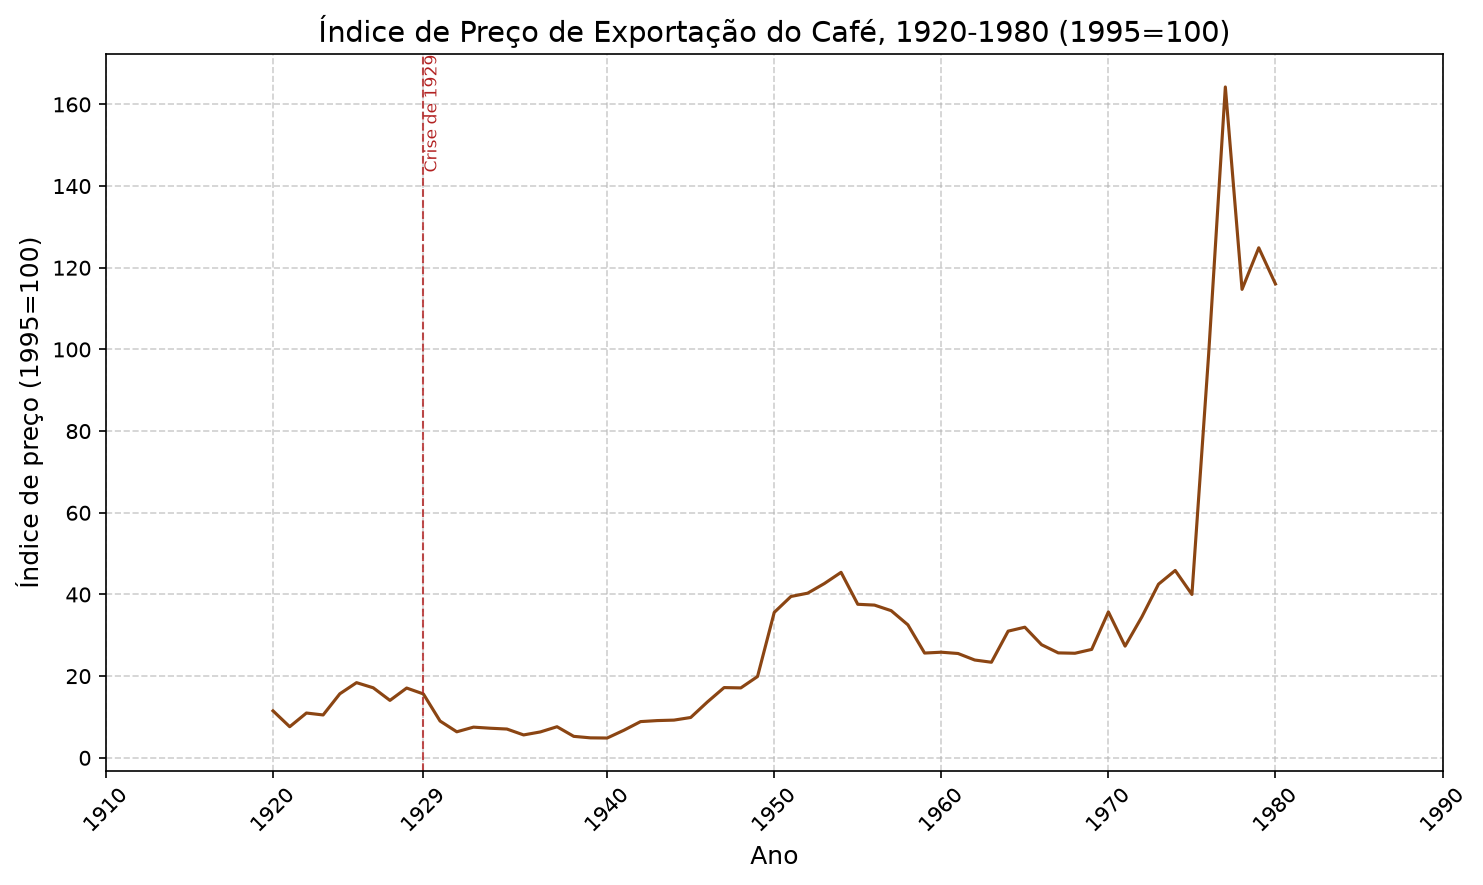
\includegraphics[width=\linewidth]{figures/cap04/preco_cafe_1920_1980.png}
\caption{Índice de preço do café, 1920--1980}
\label{fig:cap04-preco-cafe-1920-1980}
\aiflag{(fonte)}
\end{figure}

Na prática, portanto, o Plano de Metas foi levado a frente sem um
desenho claro de como financiá-lo \citep{abreu_ordem_2014}. Os custos nacionais foram
40\% da União, 10\% dos estados, 35\% de empresas privadas e estatais e
15\% de entidades públicas (BB, BNDE, etc.); já os recursos internacionais
vieram de entidades de crédito (Eximbank norte-americano e Banco
Mundial), entidades oficiais estrangeiras, investimentos em importações
sem cobertura cambial e ``suppliers' credits''; sem reforma tributária,
o financiamento público exigiu severos déficits, na prática, financiando
o programa com inflação resultante da expansão monetária e do crédito
\citep{villela_dos_2025}.

Apesar da centralidade do poder público, via tesouro e estatais, o plano
também continha mecanismos de incentivo ao capital privado. Estes eram
principalmente a proteção contra importações em setores com
``similares'' nacionais, a oferta de crédito subsidiário pelo Banco do
Brasil e BNDE, além de autorização de empréstimos no exterior para
empresas. \citep{abreu_ordem_2014}. Já o sistema cambial, que subsidiava importação de
bens de capital e insumos básicos, era complementado pela proteção
aduaneira. Dentre o conjunto de metas, a ligada à construção de
ferrovias, a refino de petróleo e ao carvão tiveram o pior desempenho, o
melhor foi a meta ligada a construção de rodovia, que ultrapassou em
38\% o objetivo (Viela). \aiflag{citação informal e com erro de digitação (``Viela''); provavelmente \citep{villela_dos_2025}, já usado corretamente em outros pontos do capítulo -- ajustar para o comando \textbackslash citep padrão.}

No cerne da disputa estava a problemática política. Não é que o governo
JK não considerasse a inflação um problema, mas conciliar seu combate
com as demandas tanto de um empresariado que demandava crescimento e
financiamento, como de uma população que buscava ascender em poder de
consumo exigia escolher prioridades. Na fórmula de JK os déficits eram
necessários diante do cenário político e a emissão monetária era a base
da cobertura destes, especialmente, pois a emissão de títulos públicos
era restrita diante de uma taxa de juros oficial baixa com vistas
justamente a estimular o investimento industrial \citep{abreu_ordem_2014}. Propostas de
reforma tributária tão pouco eram possíveis diante do desgaste político
\citep{villela_dos_2025}.

A política monetária enfrentava problemas não apenas no volume de
déficit a ser coberto, mas também nos instrumentos para tal. A começar,
até 1964 o Brasil não dispunha de Banco Central, suas funções sendo
divididas entre SUMOC e Banco do Brasil. Este acabava por operar tanto
como banco central como banco privado, o que propiciava significativa
expansão dos meios monetários. De forma simplificada, o crédito
oferecido pelo Banco do Brasil aos demais bancos era contabilmente
registrado como reserva neste - pois ele centralizava o sistema bancário
- permitindo expansão monetária irrestrita \citep{abreu_ordem_2014}. Ao mesmo tempo, a
perspectiva de controle de custos de vida e também dos custos
industriais implicava em enorme déficit com o sistema ferroviário e
dificuldades de conter gastos com funcionalismo público \citep{abreu_ordem_2014}.

É importante discutir brevemente a questão dos investimentos
estrangeiros e seu papel no Plano de Metas. No centro da problemática
está a contradição inerente ao modelo de substituição de importações
onde o avanço da produção nacional produz ele mesmo um crescimento da
demanda de importação tanto de matérias-primas e peças, como de máquinas
e equipamentos necessários a novas etapas da reorganização produtiva
\citep{tavares_da_1973}. Assim, o sistema baseava-se em ciclos onde breves alívios das
contas externas eram seguidos de constrições na capacidade de importar,
o que particularmente se observou entre 1957 e 1959 \citep{abreu_ordem_2014}.

Portanto, para além do investimento Estatal e nacional, o plano de metas
sempre utilizou de recursos para atrair o investimento estrangeiro e
tornar este possível mesmo ante a falta de cobertura cambial \citep{abreu_ordem_2014}.
Não à toa nos setores de bens duráveis e de capital, os que mais
cresceram durante o plano, a taxas de 18,2\% e 20,3\% em média e
dobrando sua participação na indústria nacional, concentraram fortemente
os investimentos estrangeiros \citep{villela_dos_2025}. Daí a formação de um setor
automotivo ligado a montadoras estrangeiras e de um setor de autopeças
nacional -- de menor intensidade tecnológica e de capital -- associado
às mesmas \citep{villela_dos_2025}.

Essa espécie de ``divisão de tarefas'' é o que Evans \citeyearpar{evans_dependent_1979}
vai interpretar como uma característica de nosso processo de desenvolvimento dependente.
O capital nacional fica associado a setores menos intensivos em
tecnologia e de menor crescimento, o Estado assume setores custosos e de
retorno incerto e o capital estrangeiro assume os setores de crescimento
mais rápido.

Esse privilégio ao capital estrangeiro se reflete inclusive na política
cambial e contrasta com o diagnóstico de um Brasil ``protecionista''.
Certamente havia altas taxas de importação, mas essas eram
flexibilizadas de forma discricionária. Esse processo precedia inclusive
JK. A instrução 113 da SUMOC, que permitia a importação sem cobertura
cambial e fora outra mudança instaurada por Gudin, no fim do governo
Café Filho \citep{villela_dos_2025}. Junto da instrução 70, que perdurou até 1964 e
substituiu o sistema de licenças pelo sistema de leilões, na prática,
subsidiaram o capital estrangeiro, que trazia máquinas e bens a uma taxa
de câmbio de mercado livre (mais elevada) e emitia remessas a uma taxa
de câmbio para exportações, sobrevalorizada \citep{villela_dos_2025}. A reforma cambial
em 1957 visava expressamente facilitar a importação de bens vistos como
essenciais -- cujo elenco seria feito pelo Conselho de Política
Aduaneira -- e os dispositivos de estímulo à produção nacional tinham
desenho para não encarecer as importações necessárias  \citep{abreu_ordem_2014}.

As dificuldades de financiamento interno se somavam aos empecilhos no
financiamento externo. Além do Brasil, continuar não representando
prioridade, a crescente dívida externa gerava pouca disposição por parte
do FMI de ampliar a linha de crédito brasileira. JK chegou a propor uma
tentativa de estabilização monetária em 1958, unindo esforços da fazenda
e do BNDE, a época presidido por Roberto Campos \citep{villela_dos_2025}. O problema foi
que, em meio a pressão do Congresso, a proposta de Campos e Lucas Lopes,
ministro da Fazenda, era mais gradual do que desejava o FMI. Iniciado em
1959, o ``Plano de Estabilização Monetária'' (PEM) terminou com o
rompimento de JK com o FMI em meio a dificuldades de negociação. Assim,
os incentivos políticos e econômicos do período produziram uma
manutenção quase exclusiva da característica desenvolvimentista do
governo JK, que só perderia força a partir da crise de 1961 em diante
\citep{abreu_ordem_2014}.

Em um todo, o período Juscelino viu queda de 15\% das exportações e
aumento de 50\% da dívida externa; o déficit da união era de cerca de
1/3 das receitas; entre 1958 e 1960 a inflação atingiu 24,4\%, 39,4\% e
30,5\% \citep{villela_dos_2025}. Como resultado do Plano de Metas, o PIB
cresceu a cerca de 9,3\% ao ano, 5,1\% per capita (muito acima da meta
do governo de 2\%) e a inflação média foi de 23,8\% em função do déficit
público de mais de 2\% do PIB ao ano. O forte crescimento permitia o
funcionamento do sistema apesar de seus objetivos antagônicos (altos
lucros, estabilidade, custo de vida) ao amenizar tensões políticas e
sociais. O gasto público passou de cerca de 19-20\% para 23,2\% do PIB.

Da discussão acima, apreende-se como o mecanismo da dívida pública -
externa nesse momento - e a inflação foram instituições centrais para o
conflito distributivo no país em sua industrialização. O primeiro
operava para condicionar o crescimento econômico ao aval seja de
instituições multilaterais, como o FMI, seja de multinacionais que
visavam privilégios ao capital estrangeiro. Aprofundar assim a
dependência brasileira em relação ao capital estrangeiro. Já a inflação
recompensava as elites locais, como uma forma de
concentração de renda, na prática, comprimindo os custos relativos do
trabalho frente ao capital, pois permitia uma transferência de renda de
trabalhadores - que tinham mais dificuldades em manter salários
competitivos com a inflação - para empresas e investidores, que
absorviam os reajustes de preço em seus lucros \todouser{}{citar malan}.

Essa é uma face do conflito de classe estruturado com base numa
sociedade profundamente desigual, numa economia dual como diria Prado Jr.
\citep{pradojunior2012}, mas que mantinha uma organização política democrática. Assim,
apesar de eficiente, o mecanismo estava longe de representar o ideal
para as classes capitalistas e exigia algum grau de compromisso com a
classe trabalhadora. Como já sugerido acima, o que tornava o sistema
mais estável era a perspectiva de forte crescimento econômico, quando
este passa a ser ameaçado a disputa distributiva se traduz em rompimento
com o modelo democrático.

O fato das classes trabalhadoras obterem uma melhor fatia da renda
nacional fica visível quando comparamos o volume de empregos e salário
(tabela abaixo), mesmo frente ao crescimento populacional. Como será
visto posteriormente, essa equação muda radicalmente durante a ditadura
militar, onde tanto em períodos de crescimento fraco como acelerado foi
possível comprimir o custo de reprodução da classe trabalhadora. Assim,
em que pesem contradições e limites, o processo de industrialização
ocorrido durante o período democrático, com ênfase no segundo governo
Vargas e no período JK, foi marcado por significativa melhora para a
população no que concerne sua inserção dentro da dinâmica de acumulação
vigente.

A partir de 1961, a forte queda do crescimento econômico e a crise
inflacionária colocam o sistema sob tensão. A primeira resposta foi a
tradicional receita de austeridade, como muitas vezes será repetido,
esta se articulou com uma pauta conservadora e de caráter moralista,
representada na figura de Jânio Quadros, que venceu a eleição
presidencial de 1960. Como marco da força que o movimento trabalhista
tinha alcançado, João Goulart foi eleito vice, mesmo em face do cenário
de crise.

Vale dizer, JK não podia concorrer a um segundo mandato pelas regras da
época, mas esperava retornar politicamente vitorioso em 1965, parte do
que o motivava a não fazer um ajuste fiscal significativo ao fim de seu
governo e deixar de ``herança'' seus custos políticos para o sucessor
(Villela, 2025, Mesquita, 2014, Fausto) \aiflag{citações informais em parênteses ao longo deste parágrafo e dos seguintes (``(Villela, 2025, Mesquita, 2014, Fausto)'', ``(Mesquita, 20214)'' -- ano com erro de digitação --, ``(Mesquita, 2014)'') deveriam usar os comandos \textbackslash citep/\textbackslash citeyearpar padrão do capítulo; as chaves corretas parecem ser villela\_dos\_2025 e mesquita\_inflacao\_2014, já usadas assim em outros pontos (ex.: linhas com \textbackslash citeyearpar\{vianna\_o\_2025\} e \textbackslash citeyearpar\{mesquita\_inflacao\_2014\}). ``Fausto'' permanece sem entrada correspondente em references.bib, já sinalizado alhures via \textbackslash todouser.}. Seus planos são interrompidos quando Jânio opta
pela repentina renúncia e o governo Jango se torna objeto de uma crise
política.

O governo Jânio será dos mais conservadores até então, mas com significativo
apoio popular. Sua política econômica será constituída de um programa
de austeridade, ancorado na redução dos gastos públicos, na desvalorização da moeda
e na unificação do mercado de âmbito, as duas últimas através da Súmula 204 da SUMOC\citep{villela_dos_2025}.
Tais esforços eram conjugados com mudanças no sistema de importação que, se de um lado extinguiam
a necessidade  de licença prévia, de outro impunha a necessidade de cobertura cambial. Do ponto de
vista prático, entretanto, tal medida teve pouco efeito.
Como Mesquita (Mesquita, 20214) mostra, os esforços para redução do déficit comercial foram majoritariamente
garantidos a partir da redução do subsídio a itens como petróleo, trigo e derivados. Assim,
a melhoria das contas externa acaba por ter significativo custo inflacionário para a 
população.

O conjunto de medidas teve, entretanto, uma consequência imediata mais importante, impulsionar 
um novo acordo de rolagem de dívida. O serviço da dívida externa reduziu seu 
peso de 43,6\% para 32,2\% entre 61 e 62 (Mesquita, 20214). 
Ao mesmo tempo, o governo adotou uma política externa pragmática, de
distanciamento dos americanos e aproximação de Cuba, URSS e de
movimentos de descolonização da África. Diante da crise, pouco efeito do
corte de gastos e em meio a pressão inflacionária derivada da
desvalorização cambial, Jânio renuncia. (Mesquita, 20214).

O período parlamentarista que seguiu até a eleição de Goulart em 1963, foi conturbado.
Marcado por tentativas de estabilização econômica, teve como centro o conflito
entre Goulart, na presidência, e o gabinete Neves -- liderado por Tancredo Neves
eleito pelo parlamento. Essa coalizão parlamentar que de fato liderava o país, tinha propostas
excessivamente otimistas e, em meio a recrudescimento da
inflação, tentou com o programa ``Ação Emergência'' uma estratégia
contracionista (Mesquita, 2014). O governo também mantinha uma taxa diferenciada
para exportação de café, cacau e derivados, cuja diferença para o valor de mercado
era recolhida pela SUMOC como forma de auxiliar nas finanças (Mesquita, 2014).

O programa foi ineficaz para reduzir déficits ou emissão
de moeda e conflitos entre governo e congresso levaram a rejeição pelo
congresso do sucessor de Tancredo Neves, Santiago Dantas -- que defendia
postura de priorização/corte de gastos abertamente. Apesar de
tentativas posteriores de controle inflacionário, a incapacidade da
elite de escolher entre objetivos contraditórios, crescimento e combate
a inflação, além de reajustes, salarias dados pela pressão popular.
\citep[]{mesquita_inflacao_2014}. Assim, eleito em 1963, Jango assumia com problemas similares
a seus antecessores e elegia Celso Furtado como Ministro da Fazenda, responsável
por resolvê-los.

Curiosamente, o diagnóstico de Furtado não fugia muito ao que anteriormente
tinha sido proposto. Verdade seja dita, incluia dentro de seu projeto de
Plano Trianual, garantias sociais e uma proposta de reforma agrária, mas mantinha
como principal medida de contenção da inflação a redução de gastos públicos~\citep{villela_dos_2025}.
Tal dinâmica poderia ser vista, de uma perspectiva em parte cínica, como uma prova da necessidade de um
ajuste fiscal frente ao descontrole de gastos. Mas tal olhar perderia um importante detalhe:
não se tratava apenas de perceber a necessidade de cortes de gastos, se tratava de definir quem
pagaria por eles. A reforma agrária junto da distribuição de renda forma de construir um mercado interno capaz de
apoiar uma expansão da economia, constrangida pelo modelo esgotado \citep{villela_dos_2025}. Mas da mesma forma
que cortes em subsídios e aumento de tarifas públicas geravam reação em setores populares,
cortes de crédito, fim de subsídios, aumento dos compulsórios a vista e realismo cambial, todos parte do projeto
de Furtado \citep{villela_dos_2025}, geravam forte reação nos setores econômicos, como nos grandes industriais,
multinacionais e setor agrário, que juntos mantinham significativo controle político do país.

Apesar de redução do custo de rolagem da dívida, a economia teve
desempenho desapontador, tendo o crescimento caido de 9,4\% em 1960 para
8,6\% em 1961 e 6,6\% em 1962. A inflação subiu de 25,4\% para 34,7\% e
depois 501'\% em 1962. Já o crescimento industrial foi 10,6\% para
11,1\% em 1961, mas regrediu para 8,1\% em 1962. \citep{mesquita_inflacao_2014}

No congresso o centro de debates foi a respeito do controle de capitais
estrangeiros, sendo a Lei 1431, de 1962, que tornava remessas de lucros mais restritiva do que
mesmo a postura nacionalista do segundo governo Vargas, o centro do debate.
Isso, pois a lei não previa a incorporação de reinvestimentos no total de capital sobre o qual
seria calculado o percentual que poderia ser feita e remessa. Previa ainda
controles mais rígidos pela autoridade monetária.

Apesar de ter sido associada a redução do investimento estrangeiro no país, o impacto
da legislação foi menor do que o do afastamento político
dos EUA, apesar de ter contribuído para este \citep{mesquita_inflacao_2014}. Certamente não
auxiliou a reverter uma distenção política que já advinha dos governos JK e mesmo do conservador
Jânio Quadros. Assim, Jango herda uma renegociação de dívida mais complexa que, ao falhar, acaba
contribuindo par ao abandono a austeridade. Também decisivas foram as pressões pelo reajuste do
funcionalismo público e salário mínimo \cite{villela_dos_2025}. Diante da resistência as medidas
de corte Furtado volta a Sudene e o governo abandona o projeto econômica vigente.

O ano de 1963 é marcado por forte recessão industrial resultado da redução dos
investimentos. Curiosamente, diferente da ideia de uma inflação resultante da 
falta de controle fiscal, Mesquita \citeyearpar{mesquita_inflacao_2014} aponta que o período
demonstra uma incapacidade \emph{das elites políticas} -- e deve-se aqui acrescentar econômicas -- 
em enfrentar os inevitáveis custos de curto prazo para
estabilizar a economia, mas não se caracteriza como um populismo
macroeconômico devido à falta de uma margem fiscal para implementação de
medidas ``populistas''. De fato, como se observou, a estratégia primordial dos governos de
diferentes visões político-ideológicas foi a tentativa de controle de gastos e austeridade, que falharam por pressões tanto internas
como externas. Foi a ausência de força política que levou a descontinuidade dos diversos
planos de estabilização.

A combinação de inflação e fraco crescimento leva a perda de apoio
entre sindicatos e protesto de organizações patronais. Há significativa
paralisia política no executivo e legislativo, com ``fragmentação de
recursos políticos''. Havia disputa central entre ``massas urbanas
mobilizados pelo populismo'' e ``antigas estruturas de poder''~\citep[p.192]{viannavillela2015}.
Em seguida houve renúncia de Roberto Campo, a época embaixador em Washington, e fortalecimento do lobby
conservador de \todouser{IPES e IBAD}{Contextualizar} se juntando à pressão contra o governo. A
instrução 255 da SUMOC que criava compras obrigatórias de títulos públicos
sem juros por 180 dias por tomadores de recursos bancários ampliava ainda mais a insatisfação
e gerou forte reação empresarial\citep{viannavillela2015}.

Com isso cai Carvalho Pinto, Ministro da Fazenda.
A inflação atinge 80\% no fim do ano, em meio a forte desaceleração da
atividade industrial e emerge uma onda de greves. Goulart, que tentara manter equilíbrio
entre setores da esquerda ``radical''~\citep[p.163]{viannavillela2015} e 
forças conservadoras ou visando reabrir negociações com FMI e
credores, se vê sem o apoio necessário. Manifestações tanto da esquerda 
como setores conservadores aumentam a
agravam a crise política \citep{mesquita_inflacao_2014,villela_dos_2025}, 
culminando no golpe de estado de 1964.

\todouser{}{inserir dreifus}

\begin{esboco}
Análise

Mudanças na tecnocracia

Permite processos de concentração de renda e internaliza dívida externa
(tornada pública)

Ausência de absorção de tecnologia, ausência de critérios para política
industrial

Ausência de ganhos de produtividade $\rightarrow$ reserva de mercado para as elites

Cria mecanismo de financeirização que transforma elite industrial em
financeira $\rightarrow$ mecanismo de acumulaçao de capital que mantém desigualdade
da ditadura, mesmo na crise inflacionária

Enfraquecimento da classe proletária $\rightarrow$ modifica as relações na
democracia

O sucesso da ditadura $\rightarrow$ fim do modelo político trabalhista clássico,
emerge novo populismo redistributivista

Lula apenas vence quando classe proletária e industrial estava reduzida,
explica política de esquerda distributivista e não pró desenvolvimento

COMPARAR AS INDUSTRIAS QUE CRESCRERAM ENTRE 1914-1925 com 1929-1939 e
1939-1945

IBGE | Estatísticas do Século XX | Estatísticas Econômicas | Tabelas Setoriais | Indústria\footnote{Fonte de dados: \url{https://seculoxx.ibge.gov.br/economicas/tabelas-setoriais/industria.html}}

COMPARAR PARTICIPAÇAO DA IND nos anos1 914-1925 com 1929-1939 e
1939-1945

IBGE | Estatísticas do Século XX | Estatísticas Econômicas | Contas Nacionais\footnote{Fonte de dados: \url{https://seculoxx.ibge.gov.br/economicas/contas-nacionais.html}}

COMPARAR DADOS DA ACUMUlAÇÂO BRUTA de capital

Participáção da administração pública em máquinas e equipamentos

Movimento das importações
\end{esboco}

\subsection{Balanço Estatístico Comparar período 1892-1930 e posterior a 1930}\label{balanuxe7o-estatuxedstico-comparar-peruxedodo-1892-1930-e-posterior-a-1930}

\begin{esboco}
População e demografia, , força de trabalho

PIB vs PIB industrial

Crescimento do pessoal ocupado / Part na população ativa (ext. Vs
transformação)

Crescimento dos estabelecimento / extrativa vs transformação

Produção industrial (extrativa vs transformação)

Pauta exportadora / participação da industria

Pauta importadora / participação dos diferentes bens

Setores industriais em ascenção / Participação dos setores

Produtividade do trabalho (geral vs industria)

Dívida externa (valor total e credores)

Inflação acumulada

Malha ferroviária e fornecimento de energia

Urbanização e setor de construção civil
\end{esboco}

\subsection{Balanço estatístico}\label{balanuxe7o-estatuxedstico}

\subsection{Comparar período de 1930 até 45 (aprox) com 45 até 64}\label{comparar-peruxedodo-de-1930-atuxe9-45-aprox-com-45-atuxe9-64}

\begin{esboco}
População e demografia, força de trabalho

PIB vs PIB industrial (e per capta)

Crescimento do pessoal ocupado / Part na população ativa (ext. Vs
transformação)

Crescimento dos estabelecimento / extrativa vs transformação

Produção industrial (extrativa vs transformação)

Pauta exportadora / participação da industria

Pauta importadora / participação dos diferentes bens

Setores industriais em ascenção / Participação dos setores

Produtividade do trabalho (geral vs industria)

Dívida externa (valor total e credores)

Inflação acumulada

Dados sobre sindicatos

Malha ferroviária/rodoviária e fornecimento de energia

Urbanização e setor de construção civil
\end{esboco}

\subsection{1964-1973: golpes e ``milagres''}\label{golpes-e-milagres}

\begin{esboco}
Comparação golpe de 64 com Vargas

Descrição geral da economia

Periodo liberal e crise

``Milagre econômico''

Dívida e câmbio

Instituições financiadoras (FMI etc)

Descrição geral da política

AI-5 e repressão

PND

Papel das multinacionais

Indústria brasileira

Estatais

Crise do petróleo

Boris

Florestan

Peter Evans

Moyama

Gambiagi

Feijo

Resumo da industrialização

\textbf{Instituições:}

Estado e centralização

Classes sociais e elites

Modelo de acumulaçao

Mercado de trabalho

Transformações técnicas

Regime cambial

Regimes de dependência e acumulação na escala global

Divida externa e financiamento internacional

Capital produtivo internacional

Regulação global do comércio (abertura comercial)

\textbf{Dimensão temporal}

Temporalidade

caráter tardio

Conjunturas críticas: concomitância com crises externas (guerras e 29)

Sequencia

Alternância externo-interno: Independencia, fim do trafico,
independencia, 1 guerra, valorização do cafe, crise 29, valorizaçao 2 e
revolução, segunda guerra, democracia

Trajetórias de Dependência geográficos

Trajetórias de dependência da escravidao

Trajetória de \sout{dependẽncia} \aiflag{dependência} da relação com economias centrais

Ritmo

gradualidade, aceleração e impulso/virada

Gradualidade nas transformações institucionais (desenvolvimentismo)

Gradualidade na formação de classes

Pontos de viradas decorrentes do acumulo de transformações
\end{esboco}